\documentclass[12pt,a4paper]{article}
\usepackage[margin=2.5cm]{geometry}
\usepackage[T1]{fontenc}
\usepackage[utf8]{inputenc}
\usepackage{amsmath,amssymb}
\usepackage{newtxtext,newtxmath}
\usepackage{graphicx}
\usepackage{float}
\usepackage{booktabs,longtable,array,tabularx}
\usepackage{placeins}
\usepackage{calc}
\usepackage{enumitem}
\usepackage{xcolor}
\usepackage{xurl}
\usepackage[hidelinks]{hyperref}
\usepackage{bookmark}
\usepackage{caption}
\captionsetup[table]{position=top,skip=6pt}
\newcolumntype{Y}{>{\raggedright\arraybackslash}X}
\usepackage{amsmath,amssymb}
\usepackage{siunitx}

\sisetup{
 table-format=2.2,
 round-mode=places,
 round-precision=2
}

\setcounter{secnumdepth}{3}
\setcounter{tocdepth}{3}
\providecommand{\tightlist}{\setlength{\itemsep}{0pt}\setlength{\parskip}{0pt}}
\setkeys{Gin}{width=\linewidth,height=0.82\textheight,keepaspectratio}
\hypersetup{
  pdftitle={LiDAR-Based Occlusion Metrics for 3D Object Detection},
  pdfauthor={Riley So},
  colorlinks=true,
  linkcolor=black,
  citecolor=black,
  urlcolor=blue
}
\title{LiDAR-Based Occlusion Metrics for 3D Object Detection\\[1em]\large Preliminary Report}
\author{Riley So\\Supervisor: Mao Shan}
\date{2026}

\begin{document}
\begin{titlepage}
\centering
{\LARGE\bfseries LiDAR-Based Occlusion Metrics for 3D Object Detection\par}
\vspace{2cm}

\includegraphics[width=0.25\textwidth]{figures/image1.png}\par
\vspace{2cm}
% {\Large final report\par}
\vspace{2cm}
{\large\bfseries Author: Riley So\par}
\vspace{1cm}
{\large\bfseries Supervisor: Mao Shan\par}
\vfill
{\large 2026\par}
\end{titlepage}

\tableofcontents

\newpage
\section{Background and Motivation}

Sensing capability and object detection are components in autonomous
driving systems. Modern vehicle datasets contain millions of annotated
objects that require consistent and reliable labelling for modern
training and evaluation. For example, the Waymo Open Dataset alone
contains over 12 million annotated labels with detailed object
attributes \cite{bib_ref_1}. Existing benchmarking criteria
often rely on subjective visibility annotations, image-based criteria or
overlook LiDAR perception quality.

LiDAR sensors perceive environments uniquely due to the geometric and
spatial nature of point cloud data. Factors such as point sparsity,
scanning angle, self-occlusion, and external occlusion can significantly
influence detection performance even when image visibility is sufficient
\cite{bib_ref_2}. As a result, current dataset difficulty
labels may overlook important LiDAR-specific perception limitations.
This thesis investigates the use of LiDAR-derived metrics to better
characterise partial occlusion and detection difficulty in urban driving
environments. By introducing a LiDAR-centred criterion, the study aims
to provide improved insight into dataset quality, perception robustness,
and model benchmarking.

\subsection{Research Question}

At comparable object ranges and LiDAR point counts, does a fine-grained, geometry-based measure of partial occlusion explain vehicle-detection difficulty better than the coarse difficulty and visibility annotations used in established autonomous-driving benchmarks?


\subsection{Aims}

This thesis aims to develop and validate a fine-grained, geometry-based measure of partial occlusion in LiDAR point clouds, and to determine whether it explains vehicle-detection difficulty better than the coarse difficulty and visibility annotations used in established autonomous-driving benchmarks.


Existing evaluation metrics describe whether and how accurately a detector succeeded; the proposed measure instead characterises how difficult the LiDAR observation was before detection. It is intended to add an object-level axis of intrinsic observability to conventional performance evaluation, enabling detector outcomes to be interpreted in relation to the geometric evidence available to the sensor.

Existing benchmarks describe detection difficulty using coarse, subjective, or image-dominant criteria, such as two-dimensional bounding-box height, truncation, and ordinal occlusion labels in KITTI. These criteria do not directly describe the geometry visible to a LiDAR sensor. Urban driving environments are selected because their clutter, dynamic objects, and complex lines of sight produce varied occlusion configurations. Reliable LiDAR perception in these conditions is important for downstream tasks including object tracking, motion planning, risk assessment, and occlusion-aware decision making.

Three aims support this goal:

\begin{enumerate}
    \item \textbf{Characterise the limitations of coarse annotations.} Quantify the variation in geometric visibility and detector difficulty within individual coarse difficulty or visibility groups while controlling for object range and LiDAR point count. This will test whether existing categories adequately distinguish object-level detection difficulty.

    \item \textbf{Define a fine-grained geometric occlusion measure.} Construct an object-level measure from sensor viewpoint, visible surface coverage, per-face visibility, and occluder geometry, while distinguishing external occlusion from self-occlusion. Ablation and sensitivity analyses will determine which geometric components provide the most informative and repeatable characterisation. Point count and point density will be retained as comparison baselines and covariates rather than embedded in the definition of occlusion.

    \item \textbf{Validate the measure against detector outcomes and existing annotations.} Determine whether the proposed measure explains per-object detection status, confidence, and localisation performance more strongly than coarse annotations, range, or point count alone. The primary validation will use the Mixed Signals V2X dataset; comparisons with KITTI, Waymo, or nuScenes will be conducted where compatible annotations, sensor geometry, and detector outputs are available.
\end{enumerate}

Ultimately, the framework aims to improve LiDAR perception benchmarking and support clearer object-level annotation standards. Extension to operational multi-agent V2X perception and roadside-unit deployment optimisation is reserved for future work.


\subsection{Scope}

The scope of this thesis is limited to the development of a framework
for quantifying partial occlusion from the perspective of an ego vehicle
in addition to other agents provided in a V2X dataset. The study focuses
specifically on LiDAR-based 3D object detection scenarios in current
datasets and does not attempt to redesign object detection models or
sensor hardware.

\section{Literature Review}

\subsection{LiDAR}

Light Detection and Ranging (LiDAR) enables the reconstruction of 3D
maps by producing high-definition point clouds and excels in depth
perception tasks, object avoidance and ranging
\cite{bib_ref_3}. LiDAR is a critical technology in
autonomous driving development because of its ability to function in
diverse lighting and weather. It provides more accurate spatial
representation than cameras, providing key data points for localisation
and tracking \cite{bib_ref_4}.

Despite its strengths in object avoidance, LiDAR can be less effective for
detailed object detection or classification, requiring fusion with
camera data, multiple lasers with different frequencies or higher beam
count. LiDAR is susceptible to occlusions, background interference, low
lighting and poor weather and is therefore often supplemented with camera sensors
that perform better in feature detection \cite{bib_ref_5}.
LiDAR systems are also limited by finite sensing range and angular
resolution and are unable to perceive through opaque objects. Like all
visual sensors, LiDAR is subject to the occlusion challenge. For
example, when a pulse strikes the first visible surface, regions behind that surface
remain unobserved. This results in an incomplete representation of the
environment which is often described as only a 2.5D scan
\cite{bib_ref_6}.

Beyond this, LiDAR is strongly influenced by sensor geometry and scene
configuration. Sparse angular resolution means long-range settings
create gaps between beams allowing partially obscured objects to be
occasionally missed. Static structures such as buildings and traffic
features create persistent occlusion zones. LiDAR occlusion introduces
temporary inconsistency, as dynamic objects move in the surrounding
previously hidden regions become visible while others remain occluded.
This problem has been approached with various techniques such as multi
frame aggregation, i.e., VADet (2024)
\cite{bib_ref_7,bib_ref_8}.

\subsection{}

\begin{table}[htbp]
    \centering
    \caption{Comparison of LiDAR geometric similarity metrics \cite{bib_ref_4}.}
    \label{tab:lidar-geometric-metrics}
    \small
    \setlength{\tabcolsep}{3pt}
    \sloppy
    \renewcommand{\arraystretch}{1.15}
    \begin{tabularx}{\textwidth}{|p{2.7cm}|p{1.1cm}|p{3.4cm}|Y|}
        \hline
        \textbf{Metric} & \textbf{Year} & \textbf{Evaluation focus} & \textbf{Characteristics} \\
        \hline
        Chamfer Distance (CD) & 1970s & Average nearest-neighbour distance between two point clouds & Computationally efficient, but sensitive to noise, translation, scale and density variation. \\
        \hline
        Earth Mover's Distance (EMD) & 1979 & Minimum cost of transforming one point cloud into another & Provides detailed one-to-one geometric comparison, but is computationally expensive and normally requires equally sized point sets. \\
        \hline
        Density-Aware Chamfer Distance (DCD) & 2021 & Geometry and local point-density similarity & Extends CD with density awareness and is comparatively robust to noise, distortion, density variation and outliers. \\
        \hline
        Iterative Closest Point (ICP) & 1992 & Alignment error after point-cloud registration & Effective for registration, but computationally expensive and sensitive to initial alignment and outliers. \\
        \hline
        Histogram-based comparison & 2000s & Distribution of pairwise point distances & Captures global structure and is robust to translation and rotation, but can require substantial memory for large clouds. \\
        \hline
        Voxel intersection over union (voxel IoU) & 2016 & Overlap between voxelised point-cloud representations & Measures spatial occupancy similarity, but depends on voxel resolution and is sensitive to misalignment. \\
        \hline
    \end{tabularx}
\end{table}

\subsubsection{Density-Aware Chamfer Distance (DCD)}

Although comprehensive of LiDAR spatial distribution, these geometric
metrics still do not explicitly quantify LiDAR-specific partial
occlusion scenarios such as point miss, self-occlusion, and external
occlusion and its effect on perception. This gap was explored by Ali et
al. \cite{bib_ref_4} in their investigation on fidelity of
simulated LiDAR.

The paper proposes a framework for quantitative comparison between real
and simulated LiDAR scans using geometric similarity metrics, where many
previous studies relied primarily on visual inspection or perception
model outputs. They evaluated Chamfer Distance, Earth Mover's Distance,
Iterative Closest Point (ICP), and Density Aware Chamfer Distance (DCD),
under degradation conditions such as noise, distortion, outliers,
orientation changes, and point density variation.

Their findings demonstrated that DCD performed the best overall as a
geometric similarity metric, having the best sensitivity under
degradation as well as computation efficiency. This metric is
significant to this thesis and is a strong potential baseline for its
sensitivity to degradation, and ability to evaluate LiDAR fidelity. For
example, scenes with dynamic objects, partial occlusion degree can be
examined and quantified with DCD.

Furthermore, the paper brings to light to the fact that geometric
similarity alone does not guarantee similar perception model outputs, as
variation in LiDAR intensity and point density distribution still
significantly influenced semantic segmentation performance
\cite{bib_ref_4}. Therefore, while DCD is effective for
quantifying geometric similarity between LiDAR scans, it does not fully
capture semantic detail, or the perception difficulty, which this thesis
aims to address.

\subsubsection{LiDAR Point Sparsity and Perception Quality}

Hu et al. proposed the Point-Density-Aware Voxel (PDV) network, a LiDAR
based 3D object detection framework that explicitly accounts for
variations in LiDAR point density within autonomous driving
environments. The study recognised perception limitations on sparse and
partially occluded scans and addressed it with novel density-aware
feature extraction methods which included voxel point centroid
localisation and density-aware RoI pooling using kernel density
estimation and self-attention mechanisms. Evaluation on the Waymo Open
Dataset and KITTI benchmark demonstrated that incorporating point
density information improved detection accuracy and reduced false
positives at longer distances compared to previous state-of-the-art
methods. The study concluded that LiDAR point density is not only a
sensing limitation but also a meaningful perception feature that can
improve robustness and reliability in 3D object detection systems.
This finding establishes point density as a LiDAR-specific feature that is relevant to perception quality \cite{bib_ref_10}.

\begin{table}[htbp]
    \centering
    \caption{Summary of commonly reported detector metrics.}
    \label{tab:detector-metrics}
    \small
    \setlength{\tabcolsep}{3pt}
    \sloppy
    \renewcommand{\arraystretch}{1.15}
    \begin{tabularx}{\textwidth}{|p{2.7cm}|p{4.1cm}|Y|}
        \hline
        \textbf{Metric} & \textbf{Evaluation focus} & \textbf{Interpretation and limitation} \\
        \hline
        Mean average precision (mAP) & Detection performance across classes and IoU thresholds & Widely used overall score, but depends strongly on the detector architecture, training data and evaluation protocol. \\
        \hline
        Intersection over union (IoU) & Overlap between predicted and ground-truth boxes & Measures localisation quality, but does not directly represent confidence, point-cloud quality or occlusion. \\
        \hline
        Precision & Correct detections as a proportion of all predicted detections & High precision indicates few false positives, but does not show how many objects were missed. \\
        \hline
        Recall & Correctly detected objects as a proportion of all ground-truth objects & High recall indicates few missed objects, including potentially sparse or occluded targets, but does not penalise false positives alone. \\
        \hline
        F1-score & Harmonic mean of precision and recall & Provides a single balance between false positives and false negatives, but depends on the selected confidence threshold. \\
        \hline
    \end{tabularx}
\end{table}

\subsection{Datasets}

Various datasets exist that provide robust training data for autonomous
vehicles in urban environments with cameras as well as LiDAR data.
Existing open datasets often contain difficulty scores for their class
labels that have criteria that vary between datasets. V2X is an emerging
category of datasets that contain sensor information from multiple
agents and are intended at benefiting collaborative autonomous vehicle tasks.

Vehicle-to-everything (V2X) perception involves the fusion of multiple
agent's viewpoints to collaborate in time on the current state of the
road; thus, views occluded from one ego vehicle can be supplemented by
the perception of other road vehicles or infrastructure. In theory, this
gives the agents a significant informational advantage as they can
perceive the scene under the context of multiple viewpoints, where one
agent's blind spot is able to be supplemented by an agent with view of
that blind spot. Therefore, V2X poses significant advantages over humans
and single perception systems where areas that are occluded are solved
by collaborative perception \cite{bib_ref_11}.

\subsubsection{Mixed Signals}

The Mixed Signals V2X dataset released in 2025 is a collection of
heterogeneous LiDAR data collected in Sydney, Australia. The dataset
featured 45.1k point clouds and 240.6k bounding boxes that were
collected from three connected autonomous vehicles and one roadside
unit. The aligned and consistent data provides a solid foundation for
occlusion metrics based on an ego vehicle
\cite{bib_ref_12}.

\subsubsection{KITTI}

The KITTI dataset, released in 2012 was a collaboration between
Karlsruhe Institute of Technology in Germany and Toyota Technological
Institute in Chicago. It was the first multimodal benchmark dataset. It
contains both stereo camera data and 64-line mechanical LiDAR and
synchronised using high-precision GPS/IMU. The dataset contains 75,000
frames of continuous point cloud sequences covering urban roads, rural
scenes and highways. Its annotations cover classifications of 8 classes,
with occlusion and classification difficulty scored with easy, medium and
hard. KITTI is widely considered one of the most robust datasets in
single vehicle object detection. Difficulty is defined by image plane
bounding box height, image occlusion level, and truncation
\cite{bib_ref_13,bib_ref_14}.


KITTI evaluates detection performance using average precision (AP), which summarises the precision--recall curve obtained by ranking predicted boxes according to confidence and matching them to ground-truth boxes using an intersection-over-union (IoU) threshold. The benchmark uses an IoU threshold of 0.7 for cars and 0.5 for pedestrians and cyclists, and reports results separately for the Easy, Moderate, and Hard difficulty levels. The current metric, denoted \(\mathrm{AP}_{\mathrm{R40}}\), averages interpolated precision over 40 recall positions; it replaced the earlier 11-point measure to provide a finer and less biased summary of performance. KITTI reports this value independently for 2D detection, bird's-eye-view detection, and full 3D detection. Accordingly, this thesis uses 3D \(\mathrm{AP}_{\mathrm{R40}}\) to evaluate the PointPillars baseline, while treating it as an aggregate detector-performance measure rather than a direct measure of LiDAR occlusion \cite{bib_ref_14,bib_ref_29}.

\subsubsection{SemanticKITTI}

SemanticKITTI introduces a LiDAR dataset that is composed of sequential
point-wise annotated labels. A key contribution is its semantic labels
where it has annotated all 22 sequences of the KITTI Vision Odometry
benchmark. The addition of point-wise semantic labels enables detailed
scene understanding for every scene. The dataset defines 28 semantic
classes, including six dynamic classes that distinguish between moving
and non-moving objects such as vehicles and pedestrians. To assess
labelling performance, they add Jaccard Index or mean intersection over
union (mIoU) \cite{bib_ref_15}. The paper also analyses
segmentation performance as a function of distance from the LiDAR
shedding light on the fact that accuracy degrades with increasing
distance due to point cloud sparsity. Also, the dataset enables
investigation for temporal perception tasks such as distinction of
moving and non-moving objects.

\subsubsection{DAIR-V2X}

DAIR-V2X was released in 2022, and published as a large-scale
multimodal, multiview dataset for cooperative autonomous driving.
The dataset came out of AIR in Beijing China. The data was collected
using vehicle--infrastructure LiDAR and camera sensors, containing 71254 LiDAR
frames and 71254 Camera frames. The annotation covered 10 object classes
with a category attribute "occlusion state'' which was denoted
``easy'', ``medium'' and ``hard'' used in the benchmarking for object
detection models \cite{bib_ref_16}.

\subsubsection{Waymo Open Dataset}

The Waymo Open Dataset is a large-scale autonomous-driving dataset containing 1,150 scenes of synchronised data from five cameras and five LiDAR sensors. Its perception labels include vehicles, pedestrians, cyclists, and signs, with LiDAR objects represented by upright seven-degree-of-freedom 3D bounding boxes \cite{bib_ref_1}. For 3D detection, Waymo reports average precision (AP) and heading-weighted average precision (APH). APH follows the AP precision--recall calculation but reduces the contribution of a matched true positive as its wrapped heading error increases, so it evaluates orientation as well as detection. The original evaluation uses 3D intersection-over-union thresholds of 0.7 for vehicles and 0.5 for pedestrians and reports results overall and by range (0--30~m, 30--50~m, and beyond 50~m) \cite{bib_ref_1}.

Waymo also assigns each evaluated ground-truth box to a difficulty level. Labels containing no LiDAR returns are ignored. A box is assigned \textsc{Level~2} when the annotator marks it as hard or when it contains at most five LiDAR points; all remaining boxes are assigned \textsc{Level~1} \cite{bib_ref_1}. Consequently, \textsc{Level~2} contains both the \textsc{Level~1} objects and the more difficult examples. This rule is reproducible and convenient, but its point-count component is coarse: the same count can arise from long range, occlusion, surface reflectivity, object size, or an edge-on viewing angle. It therefore compresses distinct geometric causes of poor observability into a single category and does not directly measure the visible fraction of an object.

Later work introduced longitudinal-error-tolerant metrics for the Waymo camera-only 3D detection benchmark. LET-3D-AP aligns a predicted box along its line of sight before computing a tolerant IoU, allowing bounded depth error during matching. LET-3D-APL then weights matched detections by longitudinal affinity, so larger corrected depth errors still receive a penalty; the L denotes longitudinal-affinity weighting rather than an additional heading term \cite{bib_ref_30}. These metrics address localization error, whereas this thesis investigates a different limitation: whether object-level geometric visibility explains LiDAR detector performance more precisely than point count, range, or a binary difficulty level alone.

\subsubsection{nuScenes}

The nuScenes dataset contains 1,000 twenty-second driving scenes recorded in Boston and Singapore using six surround-view cameras, one 32-beam LiDAR, five radars, and positioning sensors. It provides 23 annotated object categories, which are consolidated into 10 classes for the 3D detection benchmark \cite{bib_ref_18}. Unlike KITTI and the original Waymo evaluation, nuScenes does not use intersection over union (IoU) to match detections for average precision. A prediction is matched to a ground-truth object by its two-dimensional centre distance on the ground plane. Average precision is calculated above 10\% precision and recall at distance thresholds of 0.5, 1, 2, and 4~m, then averaged across the four thresholds and the 10 detection classes to obtain mAP. This reduces the sensitivity of matching to object size and orientation, particularly for small objects whose IoU can fall sharply after a modest translation error \cite{bib_ref_18}.

The nuScenes Detection Score (NDS) combines detection rate with detection quality:
\[
\mathrm{NDS}=\frac{1}{10}\left[5\,\mathrm{mAP}+\sum_{m\mathrm{TP}\in \mathrm{TP}}\left(1-\min(1,m\mathrm{TP})\right)\right].
\]
Half of the score is contributed by mAP and half by five mean true-positive errors, evaluated using 2~m centre-distance matching. These are mean Average Translation Error (mATE), the two-dimensional Euclidean centre error in metres; mean Average Scale Error (mASE), defined as one minus 3D IoU after aligning position and orientation; mean Average Orientation Error (mAOE), the smallest yaw difference in radians; mean Average Velocity Error (mAVE), the two-dimensional velocity error in metres per second; and mean Average Attribute Error (mAAE), one minus attribute-classification accuracy \cite{bib_ref_18}. NDS therefore separates several kinds of prediction error, but it remains a performance score rather than a measure of the geometric difficulty of the input.

nuScenes additionally records camera-based visibility for each annotated instance in four bins: 0--40\%, 40--60\%, 60--80\%, and 80--100\% of the object visible across the six-camera panoramic view \cite{bib_ref_31}. This field is a useful coarse occlusion proxy, but it is not one of the five NDS true-positive metrics and does not directly measure LiDAR visibility. Within a single visibility bin, objects may differ substantially in occluder geometry, range, viewing angle, reflective surface area, and the spatial distribution of LiDAR returns. Together with KITTI's ordinal occlusion labels and Waymo's point-count-based levels, the four nuScenes bins illustrate the same limitation: a small number of categories compresses a wide geometric configuration space. The object-level LiDAR metric proposed in this thesis is intended to explain detector difficulty within these coarse groups, while complementing rather than replacing mAP and NDS.

\subsubsection{ONCE (One Million Scenes)}

The ONCE dataset released in 2021 by Huawei's Noah's ark Lab. It was collected using 128-line mechanical LiDAR with a 150 m detection range and dense LiDAR
coverage per frame. ONCE introduced development of self-supervised
pretraining models by large-scale pretext tasks such as point cloud
completion and cross-model contrastive learning using unlabeled data. It
introduces 6DOF annotations including acceleration and angular velocity
allowing development for object tracking and trajectories. ONCE strongly
supports work in unsupervised domain adaptation and cross-city
generalization \cite{bib_ref_19}.

\subsubsection{Argoverse 2}

Released in 2023, Argoverse 2 emphasises long-tail scenario perception and
multi-agent interaction modelling. The dataset contains high-precision
semantic lane annotations with attributes supporting development in
trajectory predictions. The dataset introduces incorporation of
polarization characteristics in LiDAR point clouds enabling
differentiation between glass facades and metallic surfaces
\cite{bib_ref_20}.

\subsubsection{Summary of Datasets}

\begin{table}[htbp]
    \centering
    \caption{Overview of autonomous-driving datasets relevant to this thesis \cite{bib_ref_12,bib_ref_14,bib_ref_15,bib_ref_16,bib_ref_1,bib_ref_18,bib_ref_19,bib_ref_20}.}
    \label{tab:dataset-overview}
    \small
    \setlength{\tabcolsep}{3pt}
    \sloppy
    \renewcommand{\arraystretch}{1.15}
    \begin{tabularx}{\textwidth}{|p{2.3cm}|p{1.0cm}|p{2.5cm}|p{2.6cm}|Y|}
        \hline
        \textbf{Dataset} & \textbf{Year} & \textbf{Scale} & \textbf{Scene type} & \textbf{Sensor configuration} \\
        \hline
        Mixed Signals & 2025 & 45.1k point clouds; 240.6k 3D boxes & Urban V2X scenes in Sydney & Heterogeneous vehicle and roadside LiDARs; multi-agent sensing. \\
        \hline
        KITTI & 2012 & 7,481 training and 7,518 test frames & Urban, rural and highway & Cameras, Velodyne HDL-64E LiDAR and GPS/IMU. \\
        \hline
        SemanticKITTI & 2019 & 22 sequences; about 43k scans & Sequential urban driving & Semantically annotated Velodyne HDL-64E LiDAR. \\
        \hline
        DAIR-V2X & 2022 & 71,254 LiDAR and camera frames & Urban cooperative driving in Beijing & Vehicle and roadside cameras and LiDARs. \\
        \hline
        Waymo Open Dataset & 2019 & 1,150 scenes & Urban and suburban driving & Five LiDARs and five cameras. \\
        \hline
        nuScenes & 2020 & 1,000 scenes; 390k LiDAR sweeps & Boston and Singapore & One LiDAR, six cameras and five radars. \\
        \hline
        ONCE & 2021 & Approximately 1M LiDAR frames & Urban and suburban driving & 40-beam LiDAR and seven cameras. \\
        \hline
        Argoverse 2 & 2023 & 1,000 annotated scenarios & Urban driving with HD maps & Two LiDARs and seven ring cameras. \\
        \hline
    \end{tabularx}
\end{table}

\begin{table}[htbp]
    \centering
    \caption{Evaluation protocols and occlusion information in the reviewed datasets.}
    \label{tab:dataset-evaluation}
    \small
    \setlength{\tabcolsep}{3pt}
    \sloppy
    \renewcommand{\arraystretch}{1.15}
    \begin{tabularx}{\textwidth}{|p{2.5cm}|p{3.2cm}|Y|}
        \hline
        \textbf{Dataset} & \textbf{Main evaluation metrics} & \textbf{Difficulty or occlusion information} \\
        \hline
        Mixed Signals & AP/mAP-based 3D detection & No standard difficulty labels; multiple viewpoints support LiDAR occlusion analysis. \\
        \hline
        KITTI & 2D, BEV and 3D AP & Easy, Moderate and Hard based on box height, occlusion and truncation. \\
        \hline
        SemanticKITTI & mIoU for semantic segmentation & No object-detection difficulty labels; moving and non-moving semantic classes are distinguished. \\
        \hline
        DAIR-V2X & 3D detection AP/mAP & Easy, Medium and Hard occlusion states. \\
        \hline
        Waymo Open Dataset & AP and APH & Level 1 and Level 2 based partly on LiDAR point count and annotator judgement. \\
        \hline
        nuScenes & NDS and mAP & Visibility and attribute annotations rather than KITTI-style difficulty levels. \\
        \hline
        ONCE & 3D AP/mAP & No explicit difficulty labels; results are commonly analysed by range. \\
        \hline
        Argoverse 2 & 3D detection and tracking metrics & No standard difficulty labels; includes long-tail scenarios. \\
        \hline
    \end{tabularx}
\end{table}

\FloatBarrier

\subsection{LiDAR Object Detectors}

LiDAR-based 3D object detectors can generally be divided into three main
categories: voxel-based, point-based, and point voxel-based detectors.
The task is to recognise 3D object bounding boxes and assign a label.
For the nature of this research, we focus on LiDAR only detectors.

\subsubsection{PointPillars}

PointPillars is a LiDAR-only 3D object detector that organises a point cloud into vertical columns, called pillars, across the ground plane. Within each pillar, a simplified PointNet learns a feature from the points' positions, reflectance, and offsets from the pillar centre; these features are then arranged as a bird's-eye-view pseudo-image and processed by a 2D convolutional backbone and detection head to predict oriented 3D bounding boxes. This approach preserves useful information from the unordered and sparse point cloud while avoiding the computational cost of 3D convolutions. However, limiting the number of pillars and points per pillar can discard returns, and sparse, distant, or occluded objects may produce weak pillar features. PointPillars is therefore suitable as the baseline detector in this thesis because changes in its detection confidence and localisation accuracy can be compared with the proposed occlusion metric, while recognising that its outputs are also influenced by range, point density, sampling, and pillar resolution \cite{bib_ref_28}.

Voxel based detectors first convert irregular point clouds into
structured voxel grids so that convolutional neural networks can process
them efficiently. Representative methods include VoxelNet, SECOND, and
PointPillars. VoxelNet introduced the idea of voxelising point clouds
and applying 3D convolutions for feature extraction, while SECOND
improved efficiency using sparse convolutions to reduce unnecessary
computation. PointPillars further simplified the representation by
converting voxels into vertical pillars and projecting them into Bird's
Eye View (BEV) representations for faster inference. These methods are
computationally efficient and well suited for real-time autonomous
driving applications \cite{bib_ref_2}.

Point based detectors instead process raw point clouds directly without
voxelisation, preserving the original geometric structure and fine-grained spatial information. Methods such as PointRCNN, Point GNN, and
3DSSD use PointNet style architectures or graph neural networks to learn
local geometric relationships between points. These approaches generally
achieve high localisation accuracy because they avoid information loss
caused by quantisation. However, they are computationally expensive and
have higher latency due to neighbour searching and point grouping
operations \cite{bib_ref_2}.

Point--voxel-based detectors combine the strengths of both approaches.
They use voxel representations for efficient global feature extraction
while also preserving detailed point level information for refinement.
Representative methods include PV-RCNN, STD, and SA-SSD. For example, PV
RCNN combines sparse voxel convolutions with PointNet-based set
abstraction to achieve both high accuracy and efficient computation.
According to the survey, this hybrid approach has become a major trend
in modern LiDAR-based 3D object detection because it balances detection
accuracy with real-time performance requirements
\cite{bib_ref_2,bib_ref_13}.

\subsection{Occlusion}

Occlusion is a key challenge that persists in 3D object detection.
Humans can safely navigate in occluded conditions by adjusting their
behavior by anticipating risks created by occlusions, and by
leveraging semantic and geometric information of the environment. In the
context of autonomous driving, occlusions become hazardous when they hide
dynamic agents, critical infrastructure or scene context. In dense
traffic, dynamic and large vehicles like buses and trailers,
partially occlude important features and hinder detection
\cite{bib_ref_21}. Objects not only overlap in the 2D but
are also separated in depth, causing point miss, no detection or false
confidence \cite{bib_ref_22}.

Occlusion is widely recognised as a significant challenge due to both
static and dynamic sources. Pechinger et al. \cite{bib_ref_9} classify static occlusions to include
buildings, road signs, bushes and features that do not move, dynamic
occlusions are temporary objects like pedestrians, cars, trucks and
bikes. Existing literature has predominantly focused on static occlusion
scenarios; therefore, dynamic occlusion remains an important and
emerging research opportunity within autonomous driving perception
systems \cite{bib_ref_9}.


\subsubsection{Fine-Grained Image-Based Occlusion Benchmarking}

A central difficulty in evaluating robustness to partial occlusion is the absence of a consistent definition of occlusion severity. Image-based pedestrian benchmarks use incompatible groupings. Caltech estimates visible and full pedestrian boxes and defines partial occlusion as 1--35\% and heavy occlusion as 35--80\%. EuroCity Persons uses low (10--40\%), moderate (40--80\%), and strong (greater than 80\%) categories based on annotator estimates. CityPersons estimates a full-body box with a fixed width-to-height ratio of 0.41 and reports reasonable (up to 35\%) and heavily occluded (35--75\%) subsets. KITTI instead uses qualitative states such as fully visible, partly occluded, and difficult to see \cite{bib_ref_32}. These schemes are useful within their respective benchmarks, but their different thresholds and reliance on estimated hidden extent impede direct comparison. They may also combine occlusion with scale, range, illumination, weather, and other causes of non-detection.

Gilroy et al. developed a more fine-grained image-based benchmark comprising 820 pedestrian instances in 724 images, spanning 0--99\% occlusion in ten percentage bands. Occlusion was estimated using detected body keypoints, an instance mask, and a two-dimensional body-surface-area model, with difficult high-occlusion cases manually checked. Seven pretrained two-dimensional detectors were evaluated using COCO-style mAP and true-positive, false-positive, and false-negative counts at each occlusion level \cite{bib_ref_32}. Detection performance declined as occlusion increased, false negatives increased, and true-positive rates deteriorated markedly beyond 50\% occlusion. CenterNet achieved the highest overall mAP (0.533) and the strongest results up to 80\% occlusion; Mask R-CNN performed best beyond 80\%, while RetinaNet had the lowest overall mAP (0.361). SSD and SSDLite retained comparatively high true-positive rates up to 60\% occlusion, but produced approximately 100 times more false positives than Faster R-CNN and R-FCN, and approximately 16 times more than Mask R-CNN. The authors observed that false-positive counts did not appear to vary systematically with target occlusion. Their head-visibility analysis also found similar degradation trends whether the head was visible or occluded, although it did not establish statistical independence.

This study demonstrates the analytical value of treating occlusion as a fine-grained independent variable rather than only as a broad benchmark label. Its metric is nevertheless specific to two-dimensional pedestrian imagery and estimated human-body area. LiDAR occlusion instead changes which three-dimensional surfaces return points and requires separation of external line-of-sight obstruction from self-occlusion and other causes of sparsity. The present thesis therefore adapts the experimental principle, rather than the image metric itself: it stratifies detector outcomes by a continuous object-level visibility measure, compares the result with coarse annotations and conventional covariates, and tests whether performance degradation remains after controlling for range and LiDAR point count.


\subsubsection{Level of Visibility (LoV) Metric}

LoV is a novel metric which enables the comparability between junctions
and a holistic rating of the current scene's visibility level. The
methodology is based on MATLAB simulation to evaluate static and dynamic
occlusions; and uses simulated scenarios generated by Aimsun Next. The
three main steps are running traffic simulation, performing occlusion
evaluation and generating a heatmap. The occlusion evaluation is
conducted through ray tracing and detects occlusion in 2D space. Rays
are used to portray an actual ego vehicle FoV
\cite{bib_ref_9}. The study contributes a clearer taxonomy
and definition of ``occlusion'' by grouping it into defined categories of
static and dynamic. Alongside the novel metric it provides a simulation
framework for evaluating occlusion, evidence that connected vehicle
cooperation can substantially reduce dynamic occlusion, and it also
provides insight into why static occlusion persists as a challenge in
autonomous driving.

\subsubsection{Perception Entropy Based on Vehicle Grid Occupancy Probability (PE-VGOP)}

Y. He et al. formulated LiDAR deployment optimisation framework and
introduce PE-VGOP, a perception entropy metric. PE-VGOP measures
uncertainty and perceptual quality of the environment and quantifies the
visibility uncertainties. The metric is derived from projecting LiDAR
points onto top, side and front views. Each view is divided into grids;
occupancy is computed and an entropy function used to calculate entropy
over the distributions with higher entropy relating to a higher
perception coverage. The results from a deployment on KITTI show that
PE-VGOP provides faster and more accurate evaluation results than performance
evaluation computed from detection-based methods. The study uses the
metric in the optimisation algorithm for LiDAR tilt and deployment
\cite{bib_ref_23}. PE-VGOP demonstrates a promising
development for cooperative V2X and presents an effective LiDAR-based
approach for quantifying perception coverage and environmental
visibility.

\begin{table}[htbp]
    \centering
    \caption{Comparison of visibility and occlusion metrics \cite{bib_ref_9,bib_ref_23}.}
    \label{tab:visibility-occlusion-metrics}
    \small
    \setlength{\tabcolsep}{3pt}
    \sloppy
    \renewcommand{\arraystretch}{1.15}
    \begin{tabularx}{\textwidth}{|p{2.5cm}|p{1.0cm}|p{2.8cm}|p{3.3cm}|Y|}
        \hline
        \textbf{Metric} & \textbf{Year} & \textbf{Metric class} & \textbf{Method} & \textbf{Contribution and limitation} \\
        \hline
        Level of Visibility (LoV) & 2024 & Simulation-based occlusion and visibility & Ray tracing in 2D traffic simulations with static and dynamic occluders & Produces a holistic scene-level visibility score and shows the benefit of connected sensing, but does not provide an object-level LiDAR metric. \\
        \hline
        Perception Entropy based on Vehicle Grid Occupancy Probability (PE-VGOP) & 2024 & LiDAR point-distribution and perception-entropy metric & Projects LiDAR points into top, side and front grids and computes entropy from occupancy probabilities & Efficiently evaluates LiDAR coverage and deployment, but represents scene coverage rather than object-level line-of-sight occlusion. \\
        \hline
    \end{tabularx}
\end{table}

\subsection{Summary of Literature Review}

The reviewed autonomous-driving benchmarks provide valuable but coarse descriptions of detection difficulty. KITTI combines image-plane height, truncation, and ordinal occlusion labels; Waymo assigns difficulty partly from the number of LiDAR points in a ground-truth box and partly from annotator judgement; and nuScenes records visibility in four broad camera-based bins. These schemes are not directly comparable and can group together objects with different ranges, viewing angles, occluder arrangements, surface visibility, and LiDAR-return distributions. Consequently, they cannot by themselves isolate the geometric contribution of partial occlusion to detector difficulty.

A related distinction exists between input difficulty and detector performance. Evaluation quantities such as AP, APH, NDS, recall, and localisation error describe whether and how accurately a detector succeeded, but do not directly characterise the evidence available to the sensor before inference. Gilroy et al. demonstrated in the image domain that a continuous, object-level occlusion estimate reveals degradation patterns hidden by broad pedestrian-occlusion categories \cite{bib_ref_32}. However, their two-dimensional body-area formulation does not represent the three-dimensional surface visibility, line-of-sight obstruction, or self-occlusion relevant to LiDAR. DCD measures geometric discrepancy, while LoV and PE-VGOP quantify scene-level visibility or coverage; none of these reviewed approaches directly supplies the required object-level LiDAR occlusion variable for labelled 3D boxes.

The literature therefore motivates an additional repeatable measure of pre-detection geometric observability that can be compared with coarse annotations, range, point count, and point density. The proposed thesis addresses this gap by estimating external and self-occlusion at the object level and testing whether that estimate provides additional explanatory information about vehicle-detection outcomes under comparable observation conditions.


\section{Problem Statement}

Existing vehicle perception datasets commonly define detection
difficulty using coarse and image which
do not adequately reflect LiDAR sensing quality.

\section{Project Objectives}

The project has five operational objectives:
\begin{enumerate}
    \item define an interpretable object-level measure of LiDAR partial occlusion from sensor viewpoint, visible surface coverage, per-face visibility, and occluder geometry, while distinguishing external occlusion from self-occlusion;
    \item prepare reproducible sensor--object observations and a baseline 3D object-detection pipeline using the Mixed Signals V2X dataset;
    \item quantify variation in geometric visibility and detector outcomes within coarse difficulty or visibility groups at comparable object ranges and LiDAR point counts;
    \item test whether the proposed measure explains per-object detection status, confidence, and localisation performance beyond existing annotations and simpler baselines such as range, point count, and point density, using regression, uncertainty estimates, and sensitivity analyses; and
    \item assess robustness across additional LiDAR detectors or benchmark datasets where compatible annotations, sensor geometry, pretrained models, and computational resources are available.
\end{enumerate}


\section{Methodology}
\label{sec:methodology}

\subsection{Research Design}

This study develops and validates an object-level metric for partial LiDAR visibility. The metric is intended to quantify the proportion of a labelled object that is observable from a specified sensor viewpoint. It is therefore distinguished from detector accuracy and from broader measures of point-cloud quality. Range, angular sampling, point density, and detector architecture may affect perception outcomes, but they are treated as covariates or comparison baselines rather than as definitions of occlusion.

The primary experiments will use the Mixed Signals V2X dataset because it provides synchronised observations from vehicles and roadside infrastructure. Each sensor--object pair will be treated as a separate observation, allowing the same object to be compared from viewpoints with different levels of occlusion.

\subsection{Experimental Pipeline}

\begin{figure}[H]
    \centering
    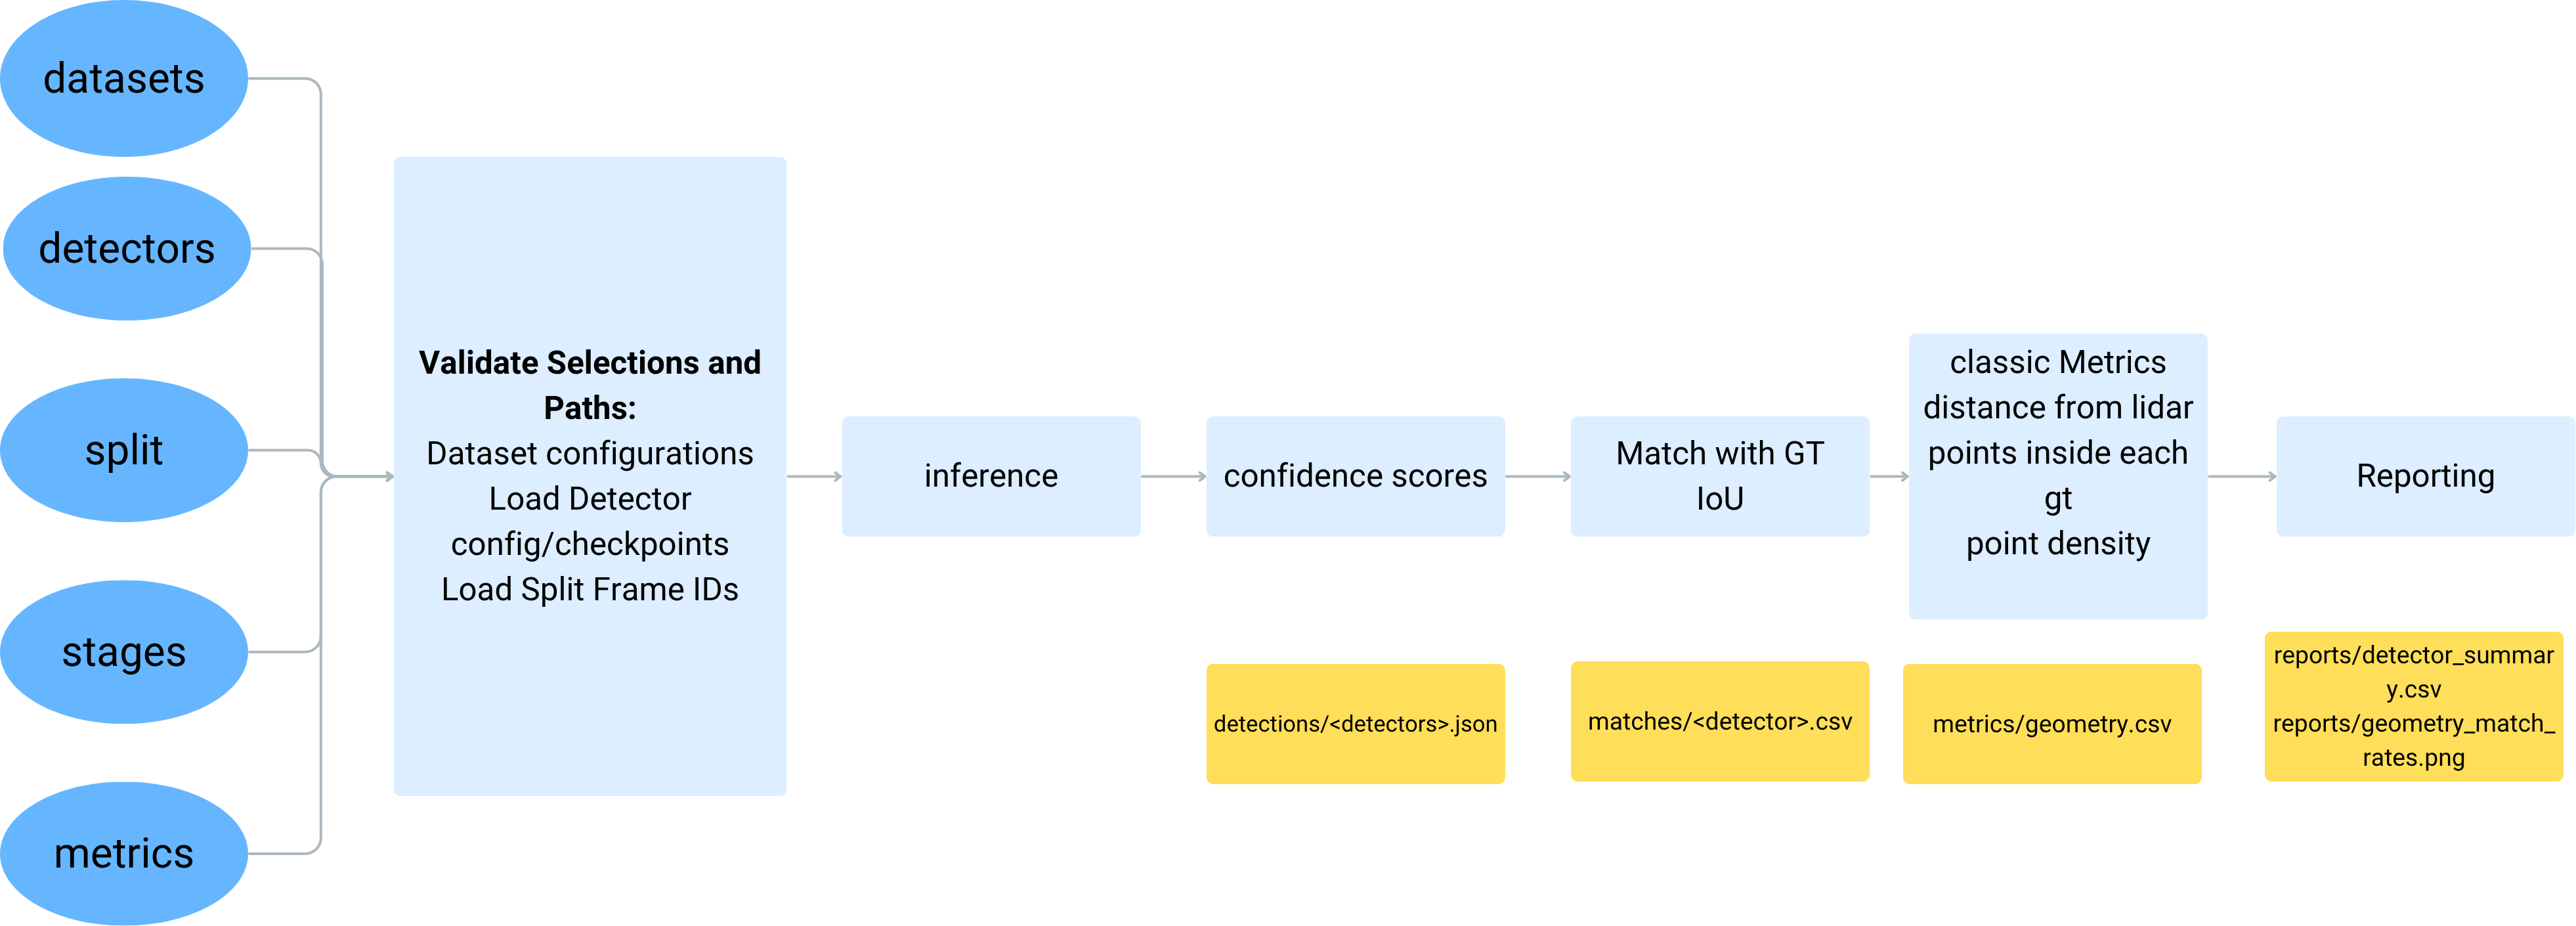
\includegraphics[width=\linewidth]{images/thesis-flow1.png}
    \caption{Proposed experimental pipeline for metric development and validation.}
    \label{fig:classic-pipeline}
\end{figure}

As shown in Figure~\ref{fig:classic-pipeline}, the pipeline comprises dataset preparation, baseline detector evaluation, occlusion-metric computation, and statistical validation. Dataset versions, coordinate transformations, class mappings, train--validation splits, preprocessing settings, detector configurations, and metric definitions will be recorded to support reproducibility.

\subsection{Dataset Preparation}

For every labelled object, LiDAR returns within the corresponding ground-truth 3D bounding box will be extracted and transformed into a common object-centred coordinate frame. The processing stage will retain the sensor pose, object pose, range, azimuth, object dimensions, class label, point count, and source agent. Quality checks will identify empty boxes, annotation inconsistencies, temporal misalignment, and points that lie close to bounding-box boundaries.

To prevent information leakage, detector selection and metric calibration will use the training partition, hyperparameter choices will use the validation partition, and final results will be reported on a held-out test partition where the dataset permits.

\subsection{Object-Level Visibility Metric}

Let $S_i$ denote the surface of object $i$ that would be observable from a sensor viewpoint in the absence of external occluders, and let $V_i \subseteq S_i$ denote the portion that remains visible after line-of-sight obstruction. The proposed visibility score is

\begin{equation}
    v_i = \frac{A(V_i)}{A(S_i)},
    \qquad 0 \leq v_i \leq 1,
\end{equation}

where $A(\cdot)$ is surface area. The corresponding occlusion score is $o_i = 1-v_i$, so larger values indicate greater occlusion.

Visibility will be estimated by ray tracing from the relevant LiDAR origin towards sampled points on the object surface. A sample is classified as externally occluded when another labelled object or reconstructed scene surface intersects the ray before the target. Surfaces facing away from the sensor will be handled separately as self-occlusion. Reporting external occlusion and self-occlusion separately will prevent two geometrically different phenomena from being hidden inside a single score.

Because observed returns also depend on range, beam pattern, incidence angle, reflectivity, and weather, raw point count and point density will not be included directly in the definition of $o_i$. Instead, they will be reported as baseline observability measures and used as covariates during validation. If sufficiently accurate surface models are unavailable, a bounding-box surface approximation will be used and documented as a limitation.

\subsection{Baseline Detector Pipeline}

A reproducible baseline will be established using an off-the-shelf LiDAR 3D object detector, such as PointPillars or SECOND, selected according to dataset compatibility and the availability of suitable pretrained weights. The detector will be evaluated using the dataset's standard protocol. Aggregate results will include precision, recall, F1-score, intersection over union (IoU), and mean average precision (mAP), where applicable.

Per-object outputs will include detection status, confidence, and localisation error. The same dataset partitions, annotation conversions, class mappings, and preprocessing steps will be used across experiments. Any unavoidable departure from an original implementation or benchmark setting will be documented explicitly.

\subsection{Validation and Statistical Analysis}

Construct validity will be assessed by testing whether increasing occlusion is associated with poorer detector outcomes. Analyses will compare the proposed score with point count, point density, range, and existing categorical difficulty labels. Detection status will be analysed using logistic regression, while confidence and localisation error will be examined using appropriate correlation or regression models. Range, object class, object size, source agent, and point density will be included as covariates where supported by the sample size.

Performance will also be reported in score bins to show whether detector degradation is monotonic. Bootstrap confidence intervals will be used to quantify uncertainty. Sensitivity analyses will examine the effects of surface-sampling resolution, bounding-box approximation, ray-intersection tolerance, and the treatment of self-occlusion.


The validation design adapts the fine-grained stratification used by Gilroy et al. for image-based pedestrian detection \cite{bib_ref_32}. Rather than reproducing their two-dimensional body-area metric or assuming that image-domain detector rankings transfer to LiDAR, the proposed continuous visibility score will be divided into sufficiently populated intervals for diagnostic reporting. Detection status, false negatives, confidence, and localisation error will be examined across these intervals; precision, recall, and AP will also be reported by interval where the sample size and evaluation protocol support them. Comparisons across more than one LiDAR detector architecture will be treated as a robustness analysis if compatible pretrained models and computational resources are available, not as a prerequisite for validating the metric.


\subsection{Evaluation Criteria and Reproducibility}

A useful metric should be repeatable, interpretable, responsive to controlled changes in visibility, and more informative about detector difficulty than point count or range alone. Reproducibility materials will include code, configuration files, dataset-conversion procedures, metric definitions, random seeds, software versions, and documented hardware requirements, subject to dataset licensing conditions.

\begin{table}[htbp]
    \centering
    \caption{Class-wise KITTI 3D $\mathrm{AP}_{\mathrm{R40}}$ (\%) for PointPillars on the complete validation split.}
    \label{tab:kitti-pointpillar-classes}
    \small
    \setlength{\tabcolsep}{3pt}
    \sloppy
    \renewcommand{\arraystretch}{1.15}
    \setlength{\tabcolsep}{3pt}
    \begin{tabular}{|l|S[table-format=2.2]|S[table-format=2.2]|S[table-format=2.2]|}
        \hline
        \textbf{Class} & {\textbf{Easy}} & {\textbf{Moderate}} & {\textbf{Hard}} \\
        \hline
        Car        & 87.76 & 78.39 & 75.19 \\
        \hline
        Pedestrian & 57.33 & 51.50 & 46.92 \\
        \hline
        Cyclist    & 81.57 & 62.95 & 58.96 \\
        \hline
    \end{tabular}
\end{table}

\subsection{Adaption of Gilroy Occlusion Benchmark as a Baseline}

This study adapts the methodology of Gilroy et al., The Impact of Partial Occlusion on Pedestrian Detectability,
 from image-based pedestrian detection to 3D LiDAR detection. Gilroy et al. assembled 820 pedestrian instances and
 assigned each instance to one of ten fine-grained occlusion intervals, ranging from 0–9% to 90–99%, with at least 55
 instances in every interval. Their occlusion estimate was based on the visible proportion of the pedestrian’s
 two-dimensional body surface, using semantic body parts and image segmentation rather than subjective labels such as
 “partly occluded.” Detector performance was then evaluated using COCO-style mean Average Precision over
 Intersection-over-Union thresholds from 0.50 to 0.95, together with true-positive, false-positive and false-negative
 behaviour at each occlusion level. The present study retains this binning structure, minimum sample requirement and
 evaluation approach, but replaces RGB images, two-dimensional body area and image detectors with KITTI point clouds,
 three-dimensional geometry and OpenPCDet detectors.

 KITTI does not provide pedestrian surface meshes, LiDAR-visible body-part annotations or ground-truth head
 locations. Consequently, the pedestrian’s oriented 3D bounding box was used as the closest consistently available
 approximation of its full three-dimensional extent. The box surfaces facing the LiDAR were identified from their
 outward normals relative to the sensor origin. Each visible face was sampled using a 30 × 30 grid, and every sample
 was weighted by the physical area represented by that grid cell. This prevents a large face and a small face from
 contributing equally merely because they contain the same number of samples. Objective occlusion was then defined as
 the area-weighted proportion of this LiDAR-facing surface covered by a contiguous mask. The percentage is therefore
 determined from known 3D geometry rather than detector output, observed point count, KITTI’s coarse occlusion label
 or human judgement. Because the surface is discretely sampled, achieved values can differ slightly from their
 nominal targets.

 Eighty-two relatively clear KITTI pedestrians were selected from 82 distinct validation frames. Candidate
 pedestrians were required to have less than 10% naturally estimated geometric occlusion and at least 30 LiDAR
 returns inside their 3D box. Using distinct frames reduces repeated-scene dependence, while the minimum-return
 requirement ensures that progressive removal can be meaningfully applied. Candidates were sorted by ground range and
 sampled across that ordering to avoid selecting only nearby, densely observed pedestrians. Each base pedestrian was
 reused at ten nominal occlusion levels—5%, 15%, 25%, through 95%—corresponding to the same ten intervals used by
 Gilroy et al. This produced exactly 82 × 10 = 820 structured-occlusion incidents, with 82 observations in every
 interval and therefore more than the required minimum of 55. However, because each pedestrian is reused, the
 independent experimental unit remains the 82 base pedestrians rather than 820 unrelated observations.

 Structured occlusion was produced by progressively removing returns from one contiguous region of the target
 pedestrian. The occluding edge was varied between the bottom, top, left and right sides of the local pedestrian box,
 with directions cycled across base instances to avoid making the result dependent on one particular occlusion
 direction. A cutoff was chosen on the sampled box surface to approximate the requested surface-area percentage.
 LiDAR returns inside the target box and behind that cutoff were removed, while the remainder of the frame was left
 unchanged. This design does not insert a simulated physical object or synthetic returns from an occluder. It instead
 represents the loss of contiguous target visibility while preserving the original road, background and surrounding
 scene. This makes the intervention reproducible and prevents changes to the scene context from becoming an
 additional uncontrolled variable, although it is not a complete physical simulation of LiDAR–occluder interaction.

 Distance and pose are controlled through the repeated-measures design: the same pedestrian, frame, orientation and
 3D box are used at every occlusion level. Point density requires an additional control because increasing occlusion
 necessarily removes target returns. For every structured sample, a matched random-removal sample was therefore
 generated by removing exactly the same number of target points, but selecting them uniformly rather than as a
 contiguous region. The controlled dataset consequently contains 820 structured incidents and 820 equal-count random
 controls. A difference between these conditions cannot be explained by distance, pose, scene or retained
 target-point count. If structured removal causes a larger performance reduction than random thinning, this supports
 the hypothesis that the spatial arrangement and surface coverage of LiDAR returns affect detection independently of
 point quantity alone.

 The modified point clouds are reconstructed during inference rather than stored as 1,640 duplicated Velodyne files.
 Each manifest entry records the original KITTI frame, target pedestrian, 3D box, occlusion level, direction, random
 seed and retained point count. The corresponding original Velodyne scan is loaded, the recorded transformation is
 reapplied deterministically, and the resulting points are passed through the normal OpenPCDet preprocessing and
 inference pipeline. This preserves reproducibility while avoiding a large redundant dataset copy.

 Detector performance is evaluated using a three-dimensional adaptation of COCO mAP. Predicted and ground-truth
 oriented 3D boxes are compared at IoU thresholds of 0.50, 0.55, 0.60, continuing in increments of 0.05 to 0.95.
 Average Precision is calculated from confidence-ranked predictions at each threshold using 101 recall points, and
 the ten AP values are averaged. The Figure 4 vertical axis, labelled “3D mAP@0.50:0.95 (%)”, is this mean multiplied
 by 100; it is not simply the percentage of pedestrians detected. Figure 6 reports the more direct true-positive and
 false-negative percentages at 3D IoU ≥ 0.50 and a confidence threshold of 0.1, together with false positives per
 ground-truth pedestrian. Predictions matching another legitimate pedestrian in the source frame are ignored rather
 than incorrectly counted as false positives for the selected target.

 A separate natural KITTI benchmark was also retained as an external realism check. All 3,769 KITTI validation frames
 were examined, of which 824 contained at least one labelled pedestrian, producing 2,280 pedestrian instances.
 Natural geometric occlusion was estimated by casting rays from the LiDAR to sampled target-box surfaces and testing
 whether another annotated 3D box was intersected first. Every natural occlusion interval contained at least 55
 instances. This natural analysis is more representative of real scenes but remains vulnerable to distance, density
 and scene-composition confounding; the controlled repeated-measures benchmark is therefore the primary experiment
 for isolating the effect of occlusion.

 The implementation remains an adaptation rather than an exact reproduction. Gilroy et al. used semantic body regions
 and actual head visibility in RGB images, whereas this study uses a bounding-box surface and defines the upper 20%
 of that surface as a head proxy. Unlabelled walls, poles and vegetation are not represented by the natural
 annotated-box visibility calculation. At very high controlled occlusion levels, all observed target returns may be
 removed, causing the structured and equal-count random conditions to converge. Finally, the current complete plots
 include PointPillars, SECOND, PointRCNN and PV-RCNN. CenterPoint and Part-A2 lack compatible local KITTI
 checkpoints, while the available Voxel R-CNN checkpoint was trained for Cars only. A full seven-detector comparison
 must not be claimed until pedestrian-compatible versions of those three models are trained or obtained using the
 same KITTI training data.

 \begin{figure}[h]
     \centering
     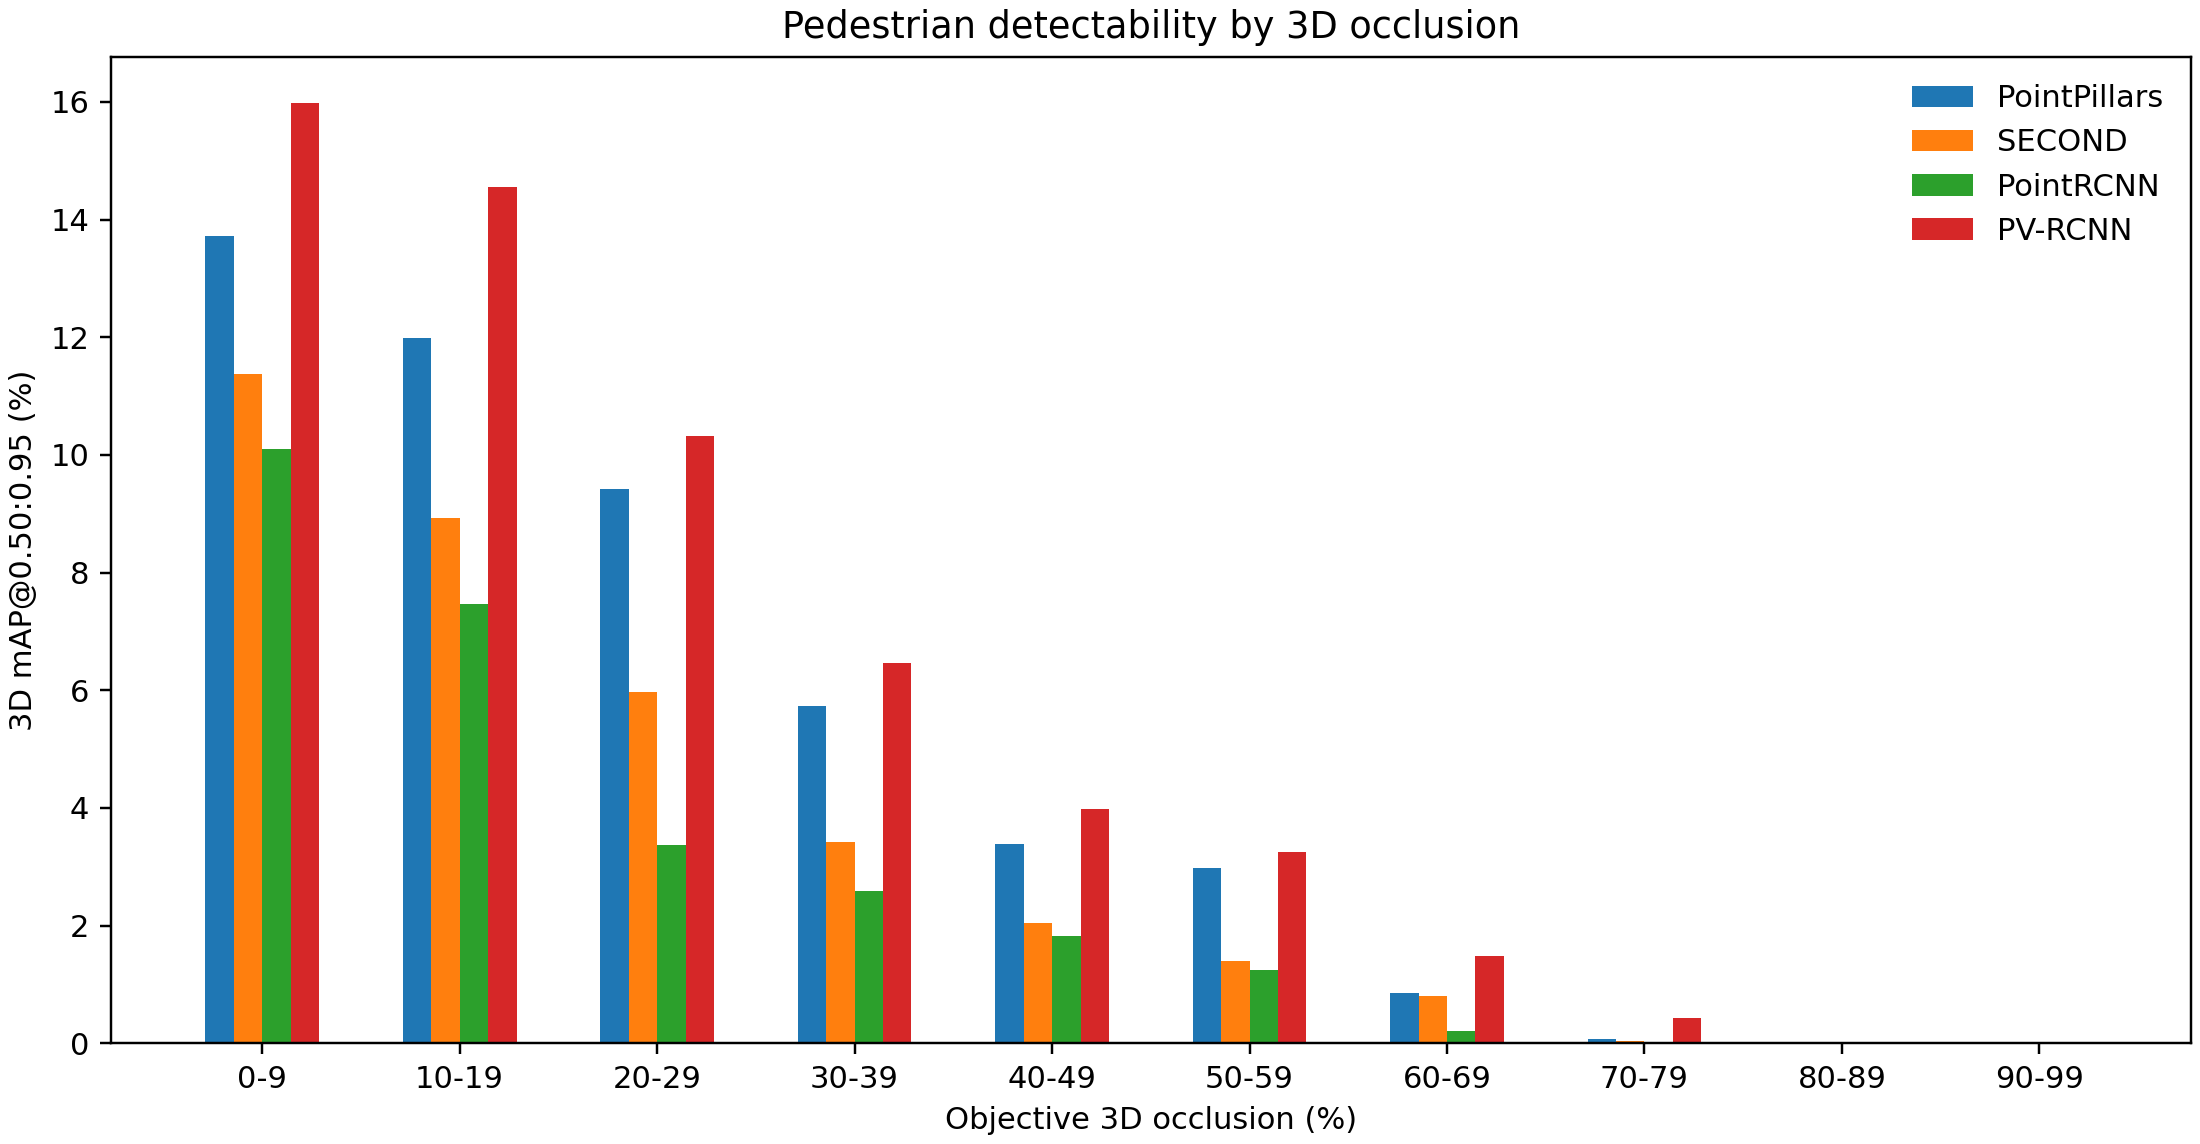
\includegraphics[width=1\linewidth]{images/map-vs-occlusion-baseline.png}
     \caption{mAP vs Occlusion}
     \label{fig:mAP vs Occlusion}
 \end{figure}

\section{Progress Report and Revised Gantt Chart}

\subsubsection{Progress}

To date, progress has focused on two components: a comprehensive
literature review and preliminary experimentation with the Mixed Signals
dataset.

The literature review surveyed LiDAR sensing characteristics, existing
dataset benchmarking criteria, occlusion quantification methods, and
relevant geometric metrics, establishing the research gap that motivates
this thesis.

In addition, initial work has been conducted using the Mixed Signals
dataset devkit. This has involved familiarisation with the dataset
structure, point cloud visualisation, and exploration of ground truth
bounding box annotations. As shown in Figure~\ref{fig:mixed-signals-occlusion-heatmap}, a preliminary heatmap
colour scheme has applied to labelled objects from an ego vehicle
perspective, visually distinguishing occluded objects by their
observability. This provides a foundation for the proposed occlusion
metric development in the next steps.

\begin{figure}[H]
    \centering
    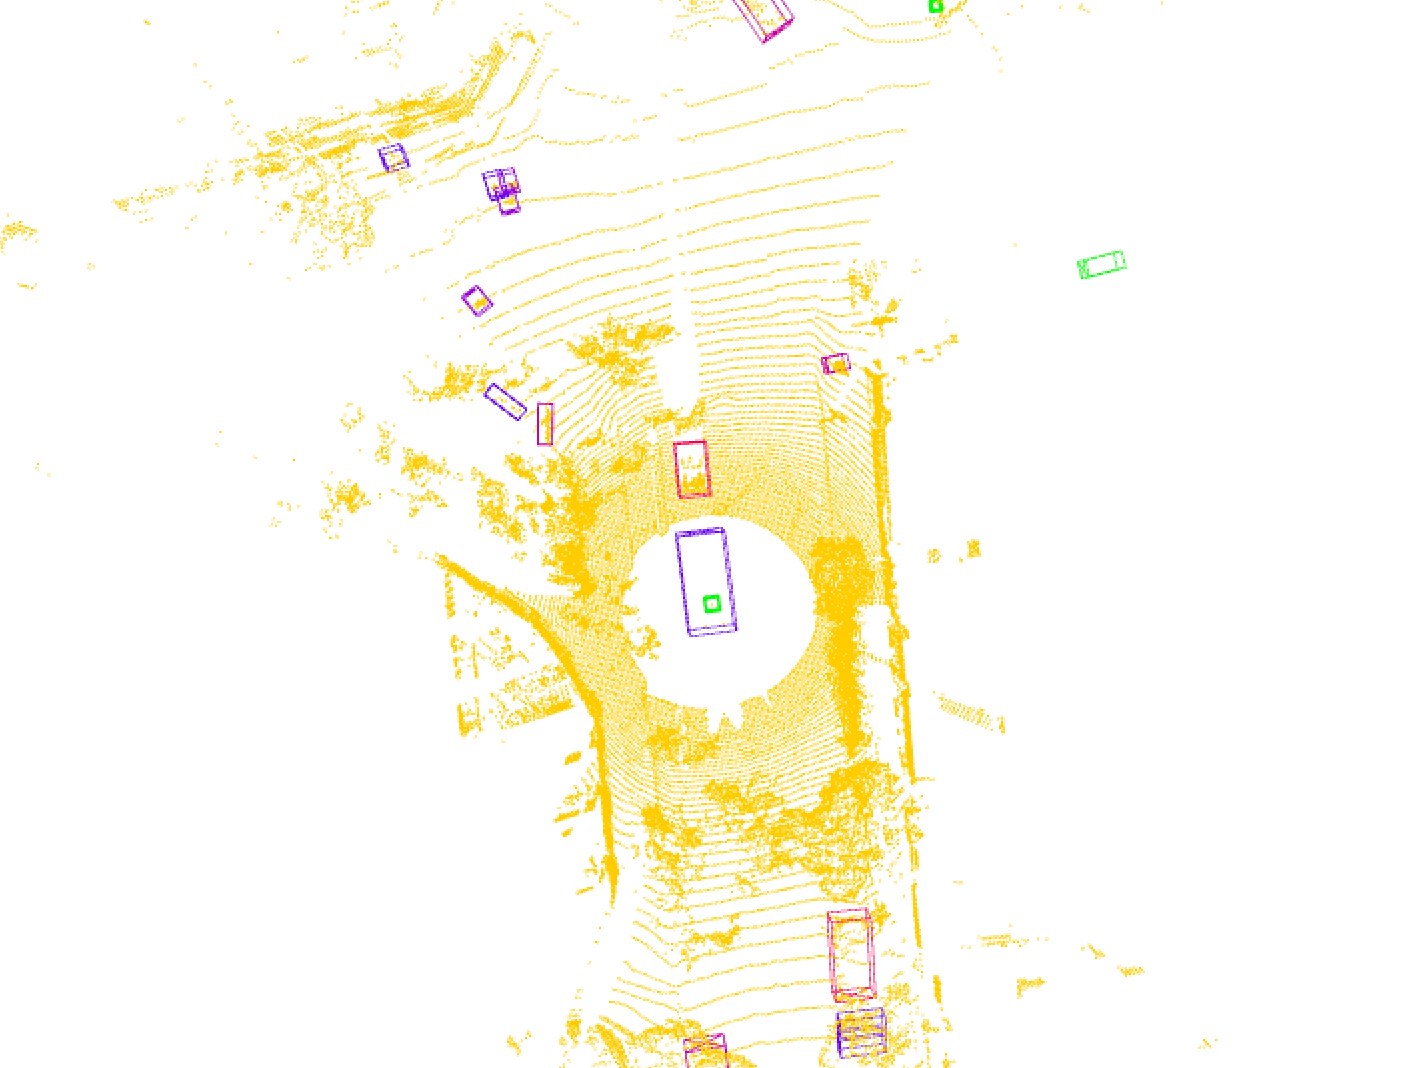
\includegraphics[width=0.44\textwidth]{figures/image8.png}
    \hfill
    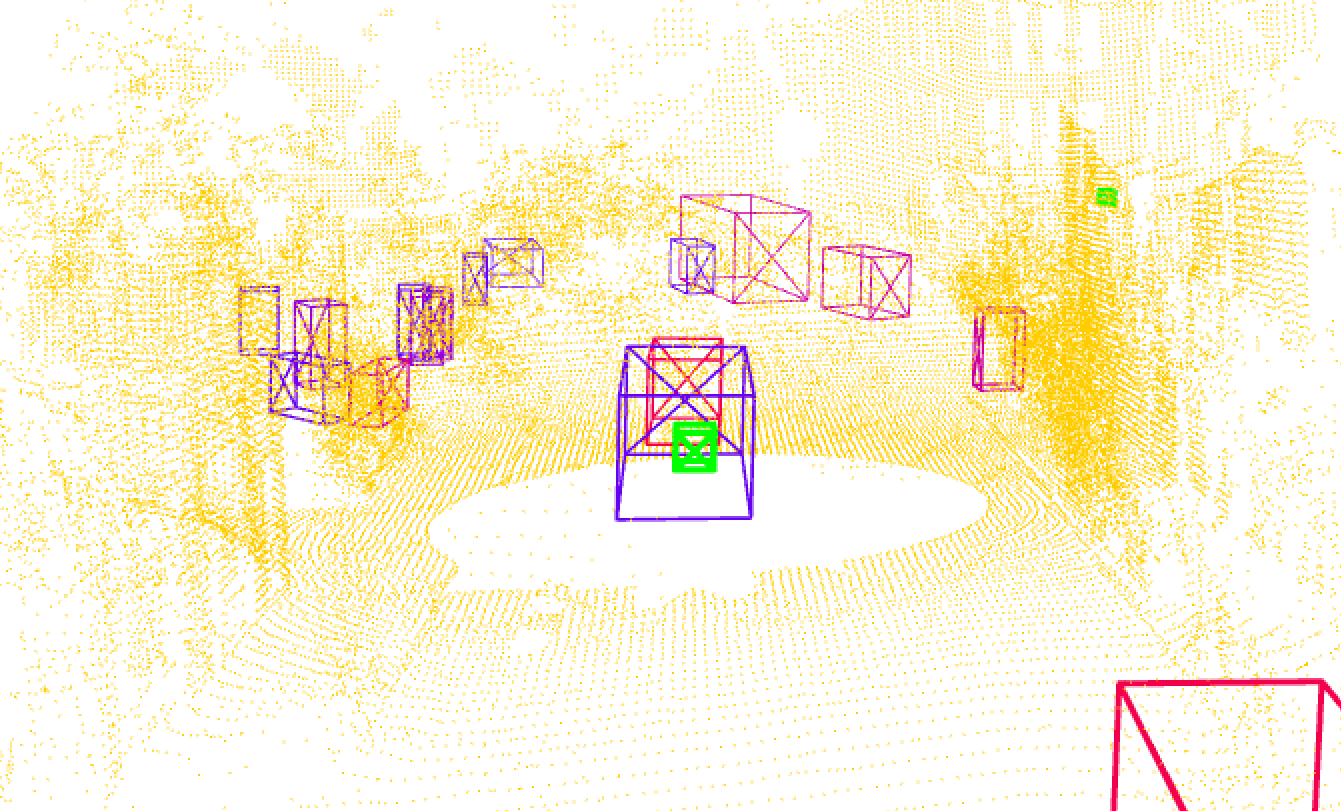
\includegraphics[width=0.50\textwidth]{figures/image9.png}
    \caption{Current progress using Mixed Signals, showing a heatmap colour scheme applied to occluded objects from an ego-vehicle perspective.}
    \label{fig:mixed-signals-occlusion-heatmap}
\end{figure}

\subsubsection{Gantt Chart}

\begin{figure}[H]
    \centering
    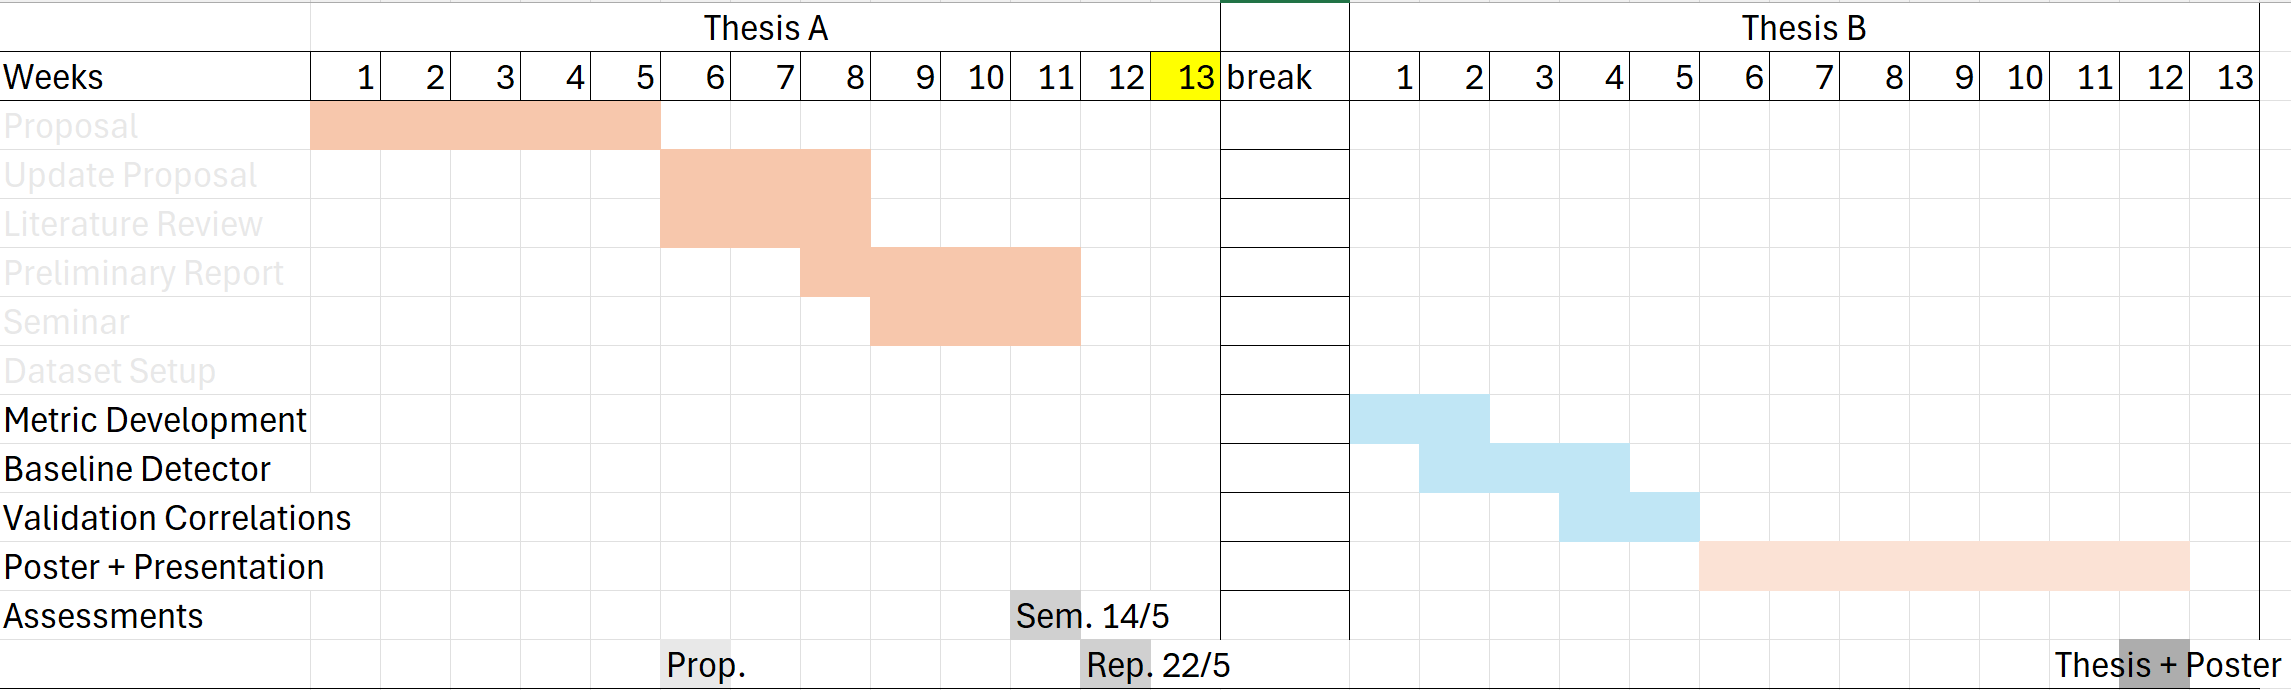
\includegraphics[width=\textwidth]{figures/image10.png}
    \caption{Revised project Gantt chart.}
    \label{fig:gantt-chart}
\end{figure}

\section{Conclusion}

Collectively, the literature points to a consistent and unaddressed
need: a quantitative, LiDAR-centred metric capable of characterising
partial occlusion at the object level. Such a metric would complement
existing difficulty annotations, provide a more physically meaningful
basis for benchmarking LiDAR object detectors, and better reflect
perceptual challenges present in complex urban driving environments.
This thesis directly addresses this gap by proposing a framework for
deriving a LiDAR-based occlusion metric from point cloud observations
within labelled 3D bounding boxes, validated against detector
performance on the Mixed Signals V2X dataset and, where appropriate, additional benchmark datasets.

\begin{thebibliography}{99}

\bibitem{bib_ref_1}\label{bib_ref_1} P. Sun \emph{et al.}, {Scalability in Perception for Autonomous Driving: Waymo Open Dataset}, in \emph{Proceedings of the IEEE/CVF Conference on Computer Vision and Pattern Recognition}, 2020, pp. 2446--2454.

\bibitem{bib_ref_2}\label{bib_ref_2} R. Qian, X. Lai, and X. Li, ``3D Object Detection for Autonomous Driving: A Survey,'' \emph{Pattern Recognition}, vol. 130, Oct. 2022. \href{https://doi.org/10.1016/j.patcog.2022.108796}{doi:10.1016/j.patcog.2022.108796}.

\bibitem{bib_ref_3}\label{bib_ref_3} D. Wang, W. Fu, J. Zhou, and Q. Song, ``Occlusion-Aware Motion Planning for Autonomous Driving,'' \emph{IEEE Access}, vol. 11, pp. 42809--42823, 2023. \href{https://doi.org/10.1109/ACCESS.2023.3268072}{doi:10.1109/ACCESS.2023.3268072}.

\bibitem{bib_ref_4}\label{bib_ref_4} S. M. Ali, T. Rahman, G. Farhani, M. H. Zaki, B. Anctil, and D. Charlebois, ``Comprehensive Assessment of LiDAR Evaluation Metrics: A Comparative Study Using Simulated and Real Data,'' \emph{IEEE Open Journal of Intelligent Transportation Systems}, 2026. \href{https://doi.org/10.1109/OJITS.2026.3673597}{doi:10.1109/OJITS.2026.3673597}.

\bibitem{bib_ref_5}\label{bib_ref_5} P. Y. Leong and N. S. Ahmad, ``LiDAR-Based Obstacle Avoidance With Autonomous Vehicles: A Comprehensive Review,'' \emph{IEEE Access}, vol. 12, pp. 164248--164261, 2024. \href{https://doi.org/10.1109/ACCESS.2024.3493238}{doi:10.1109/ACCESS.2024.3493238}.

\bibitem{bib_ref_6}\label{bib_ref_6} Q. Xu, Y. Zhong, and U. Neumann, ``Behind the Curtain: Learning Occluded Shapes for 3D Object Detection,'' 2022. [Online]. Available: \url{https://www.aaai.org}.

\bibitem{bib_ref_7}\label{bib_ref_7} J. Lin, S. Li, W. Dong, T. Matsumaru, and S. Xie, ``Long-Arm Three-Dimensional LiDAR for Antiocclusion and Antisparsity Point Clouds,'' \emph{IEEE Transactions on Instrumentation and Measurement}, vol. 70, 2021. \href{https://doi.org/10.1109/TIM.2021.3104019}{doi:10.1109/TIM.2021.3104019}.

\bibitem{bib_ref_8}\label{bib_ref_8} C. Huang, V. Abdelzad, S. Sedwards, and K. Czarnecki, ``VADet: Multi-frame LiDAR 3D Object Detection using Variable Aggregation.''

\bibitem{bib_ref_9}\label{bib_ref_9} M. Pechinger, T. Niels, and K. Bogenberger, ``Threshold Analysis of Static and Dynamic Occlusion in Urban Areas: A Connected Automated Vehicle Perspective,'' \emph{Transportation Research Record}, vol. 2678, no. 9, pp. 823--836, Sep. 2024. \href{https://doi.org/10.1177/03611981241230539}{doi:10.1177/03611981241230539}.

\bibitem{bib_ref_10}\label{bib_ref_10} J. S. K. Hu, T. Kuai, and S. L. Waslander, ``Point Density-Aware Voxels for LiDAR 3D Object Detection.''

\bibitem{bib_ref_11}\label{bib_ref_11} A. Clerigo, G. Silva, M. Schrapel, P. Rito, S. Sargento, and A. Vinel, ``Cooperative Augmented Reality: Displaying Occluded Vehicles using V2X Communications,'' in \emph{IEEE Vehicular Networking Conference (VNC)}, IEEE Computer Society, 2025. \href{https://doi.org/10.1109/VNC64509.2025.11054191}{doi:10.1109/VNC64509.2025.11054191}.

\bibitem{bib_ref_12}\label{bib_ref_12} K. Z. Luo \emph{et al.}, ``Mixed Signals: A Diverse Point Cloud Dataset for Heterogeneous LiDAR V2X Collaboration,'' Aug. 2025. [Online]. Available: \url{https://arxiv.org/abs/2502.14156}.

\bibitem{bib_ref_13}\label{bib_ref_13} X. Zhang, H. Wang, and H. Dong, ``A Survey of Deep Learning-Driven 3D Object Detection: Sensor Modalities, Technical Architectures, and Applications,'' \emph{Sensors}, Jun. 2025. \href{https://doi.org/10.3390/s25123668}{doi:10.3390/s25123668}.

\bibitem{bib_ref_14}\label{bib_ref_14} A. Geiger, P. Lenz, C. Stiller, and R. Urtasun, ``Vision meets Robotics: The KITTI Dataset.'' [Online]. Available: \url{http://www.cvlibs.net/datasets/kitti}.

\bibitem{bib_ref_15}\label{bib_ref_15} J. Behley \emph{et al.}, ``SemanticKITTI: A dataset for semantic scene understanding of LiDAR sequences,'' in \emph{Proceedings of the IEEE International Conference on Computer Vision}, 2019, pp. 9296--9306. \href{https://doi.org/10.1109/ICCV.2019.00939}{doi:10.1109/ICCV.2019.00939}.

\bibitem{bib_ref_16}\label{bib_ref_16} H. Yu \emph{et al.}, ``DAIR-V2X: A Large-Scale Dataset for Vehicle-Infrastructure Cooperative 3D Object Detection,'' in \emph{Proceedings of the IEEE/CVF Conference on Computer Vision and Pattern Recognition}, 2022, pp. 21329--21338. \href{https://doi.org/10.1109/CVPR52688.2022.02067}{doi:10.1109/CVPR52688.2022.02067}.

\bibitem{bib_ref_17}\label{bib_ref_17} R. Xu \emph{et al.}, ``WOD-E2E: Waymo Open Dataset for End-to-End Driving in Challenging Long-tail Scenarios,'' Nov. 2025. [Online]. Available: \url{https://arxiv.org/abs/2510.26125}.

\bibitem{bib_ref_18}\label{bib_ref_18} H. Caesar, V. Bankiti, A. H. Lang, S. Vora, V. E. Liong, Q. Xu, A. Krishnan, Y. Pan, G. Baldan, and O. Beijbom, {nuScenes: A Multimodal Dataset for Autonomous Driving}, in \emph{Proceedings of the IEEE/CVF Conference on Computer Vision and Pattern Recognition}, 2020, pp. 11621--11631. \href{https://doi.org/10.1109/CVPR42600.2020.01164}{doi:10.1109/CVPR42600.2020.01164}.

\bibitem{bib_ref_19}\label{bib_ref_19} J. Mao \emph{et al.}, ``One Million Scenes for Autonomous Driving: ONCE Dataset.'' [Online]. Available: \url{http://www.once-for-auto-driving.com}.

\bibitem{bib_ref_20}\label{bib_ref_20} B. Wilson \emph{et al.}, ``Argoverse 2: Next Generation Datasets for Self-Driving Perception and Forecasting,'' Jan. 2023. [Online]. Available: \url{https://arxiv.org/abs/2301.00493}.

\bibitem{bib_ref_21}\label{bib_ref_21} C. Lin, Y. Wang, B. Gong, H. Liu, and H. Liu, ``Roadside LiDAR Deployment Optimization for Vehicle-to-Infrastructure Cooperative Perception in Urban Occlusion Environments,'' \emph{IEEE Transactions on Instrumentation and Measurement}, vol. 74, 2025. \href{https://doi.org/10.1109/TIM.2025.3558231}{doi:10.1109/TIM.2025.3558231}.

\bibitem{bib_ref_22}\label{bib_ref_22} \emph{IEEE 11th International Conference on Computer Vision, 2007: ICCV 2007: Rio de Janeiro, Brazil, October 14--21, 2007}. IEEE Computer Society, 2007.

\bibitem{bib_ref_23}\label{bib_ref_23} Y. He, P. Cao, Z. Su, H. Liang, L. Zhao, and X. Liu, ``A Novel Perception Entropy Metric for Optimizing Vehicle Perception with LiDAR Deployment,'' \emph{IEEE Internet of Things Journal}, 2025. \href{https://doi.org/10.1109/JIOT.2025.3612481}{doi:10.1109/JIOT.2025.3612481}.


\bibitem{bib_ref_24}\label{bib_ref_24} S. Zhao, ``Deep 3D Information Prediction and Understanding,'' Ph.D. dissertation, School of Computer Science, Faculty of Engineering, The University of Sydney, Sydney, Australia, 2022.

\bibitem{bib_ref_25}\label{bib_ref_25} C. R. Qi, H. Su, K. Mo, and L. J. Guibas, ``PointNet: Deep Learning on Point Sets for 3D Classification and Segmentation,'' in \emph{Proceedings of the IEEE Conference on Computer Vision and Pattern Recognition}, 2017, pp. 652--660. \href{https://doi.org/10.1109/CVPR.2017.16}{doi:10.1109/CVPR.2017.16}.

\bibitem{bib_ref_26}\label{bib_ref_26} C. R. Qi, L. Yi, H. Su, and L. J. Guibas, ``PointNet++: Deep Hierarchical Feature Learning on Point Sets in a Metric Space,'' in \emph{Advances in Neural Information Processing Systems}, vol. 30, 2017.

\bibitem{bib_ref_27}\label{bib_ref_27} Y. Zhou and O. Tuzel, ``VoxelNet: End-to-End Learning for Point Cloud Based 3D Object Detection,'' in \emph{Proceedings of the IEEE Conference on Computer Vision and Pattern Recognition}, 2018, pp. 4490--4499. \href{https://doi.org/10.1109/CVPR.2018.00472}{doi:10.1109/CVPR.2018.00472}.


\bibitem{bib_ref_28}\label{bib_ref_28} A. H. Lang, S. Vora, H. Caesar, L. Zhou, J. Yang, and O. Beijbom, ``PointPillars: Fast Encoders for Object Detection from Point Clouds,'' in \emph{Proceedings of the IEEE/CVF Conference on Computer Vision and Pattern Recognition}, 2019, pp. 12697--12705. \href{https://doi.org/10.1109/CVPR.2019.01298}{doi:10.1109/CVPR.2019.01298}.


\bibitem{bib_ref_29}\label{bib_ref_29} A. Simonelli, S. R. Bulo, L. Porzi, M. Lopez-Antequera, and P. Kontschieder, ``Disentangling Monocular 3D Object Detection,'' in \emph{Proceedings of the IEEE/CVF International Conference on Computer Vision}, 2019, pp. 1991--1999. \href{https://doi.org/10.1109/ICCV.2019.00208}{doi:10.1109/ICCV.2019.00208}.


\bibitem{bib_ref_30}\label{bib_ref_30} W.-C. Hung, V. Casser, H. Kretzschmar, J.-J. Hwang, and D. Anguelov, {LET-3D-AP: Longitudinal Error Tolerant 3D Average Precision for Camera-Only 3D Detection}, in \emph{Proceedings of the IEEE International Conference on Robotics and Automation}, 2024, pp. 11886--11892. \href{https://doi.org/10.1109/ICRA57147.2024.10611526}{doi:10.1109/ICRA57147.2024.10611526}.


\bibitem{bib_ref_31}\label{bib_ref_31} Motional, {nuScenes Database Schema: Visibility}, \emph{nuScenes Devkit}. [Online]. Available: \url{https://github.com/nutonomy/nuscenes-devkit/blob/master/docs/schema_nuscenes.md}. Accessed: Sep. 3, 2026.


\bibitem{bib_ref_32}\label{bib_ref_32} S. Gilroy, D. Mullins, A. Parsi, E. Jones, and M. Glavin, {Replacing the Human Driver: An Objective Benchmark for Occluded Pedestrian Detection}, \emph{Biomimetic Intelligence and Robotics}, vol. 3, no. 3, Art. no. 100115, Sep. 2023. \href{https://doi.org/10.1016/j.birob.2023.100115}{doi:10.1016/j.birob.2023.100115}.

\end{thebibliography}


\newpage
% }\label{logbook}

\begin{longtable}[]{@{}
  >{\raggedright\arraybackslash}p{(\columnwidth - 0\tabcolsep) * \real{1.0000}}@{}}
\toprule\noalign{}
\begin{minipage}[b]{\linewidth}\raggedright
\textbf{Weekly/} \textbf{Fortnightly Log Entry}

\textbf{Project Title: Machine Learning Models using the Mixed Signals
Dataset}

\textbf{Supervisor: Mao Shan}

\textbf{Date: 08/03/2026}

\textbf{Meeting Time: 3:30 PM 2/3/2026, 29/1/2026}

Do thesis work on an applied industry problem that could only be done by
me with this one data set and with this supervisor only to get most
value.

\url{https://mixedsignalsdataset.cs.cornell.edu/download/}

MS3D++ refers to a multi sensor 3D detection and self training
framework, designed to improve 3d object performance,~

MS3D type study: \url{https://github.com/darrenjkt/MS3D}

\begin{enumerate}
\def\labelenumi{\arabic{enumi}.}
\item
  Baseline detector
\end{enumerate}

CO3 - \url{https://github.com/Runjian-Chen/CO3}

\begin{enumerate}
\def\labelenumi{\arabic{enumi}.}
\item
  \textbf{Objectives}
\end{enumerate}

\begin{itemize}
\item
  Discussed Mixed Signals and Possible paths to go down with Mixed
  Signals
\item
  Cooperative Perception, Predictive Perception,
\end{itemize}

\begin{enumerate}
\def\labelenumi{\arabic{enumi}.}
\setcounter{enumi}{1}
\item
  \textbf{Activities Performed}
\end{enumerate}

Research about 3D object detectors. Point Cloud and Lidar. Orin Nano AI
supercomputer

\begin{enumerate}
\def\labelenumi{\arabic{enumi}.}
\setcounter{enumi}{2}
\item
  \textbf{Data / Results / Plots / Diagrams / Equations}
\end{enumerate}

n/a

\begin{enumerate}
\def\labelenumi{\arabic{enumi}.}
\setcounter{enumi}{3}
\item
  \textbf{Observations and Reflections}
\end{enumerate}

n/a

\begin{enumerate}
\def\labelenumi{\arabic{enumi}.}
\setcounter{enumi}{4}
\item
  \textbf{Problems Encountered}
\end{enumerate}

n/a

\begin{enumerate}
\def\labelenumi{\arabic{enumi}.}
\setcounter{enumi}{5}
\item
  \textbf{Next Steps / To-Do List (max 50 words)}
\end{enumerate}

Research about 3D object detectors. Point Cloud and Lidar.

\begin{enumerate}
\def\labelenumi{\arabic{enumi}.}
\setcounter{enumi}{6}
\item
  \textbf{Appendices / Reference Notes (optional)}
\end{enumerate}
\end{minipage} \\
\midrule\noalign{}
\endhead
\bottomrule\noalign{}
\endlastfoot
\begin{minipage}[t]{\linewidth}\raggedright
\textbf{Weekly/} \textbf{Fortnightly Log Entry}

\textbf{Project Title: Machine Learning Models using the Mixed Signals
Dataset to For Static Mapping remove Occlusion}

\textbf{Supervisor: Mao Shan}

\textbf{Date: 20/03/2026}

\textbf{Meeting Time: 3:30 PM 20/3/2026}

Had a meeting with Steffany Berrioz and Mao Shan. I have completed the
data set visualization. We discussed that 3D image detection may not be
suitable for a thesis. There may be potential in mapping of the static
environment, and occlusion of objects. We discussed the importance of
matrix fusion, high fidelity and clean map. Coordinate system fusion.
Coordinate Frame Fusion.

\textbf{Topic: Multi-LiDAR Autonomous Exploration and Mapping for
Occlusion Removal from Point Cloud}

\begin{enumerate}
\def\labelenumi{\arabic{enumi}.}
\item
  \textbf{Objectives}
\end{enumerate}

To create a draft of the proposal by Wednesday, Submit it on Friday.

Read papers on matrix fusion.

\begin{enumerate}
\def\labelenumi{\arabic{enumi}.}
\setcounter{enumi}{1}
\item
  \textbf{Activities Performed}
\end{enumerate}

Research about 3D object detectors. Point Cloud and Lidar. Preliminary
work on partial occlusion.

Mixed Signals Devkit.

\begin{enumerate}
\def\labelenumi{\arabic{enumi}.}
\setcounter{enumi}{2}
\item
  \textbf{Data / Results / Plots / Diagrams / Equations}
\end{enumerate}

n/a

\begin{enumerate}
\def\labelenumi{\arabic{enumi}.}
\setcounter{enumi}{3}
\item
  \textbf{Observations and Reflections}
\end{enumerate}

n/a

\begin{enumerate}
\def\labelenumi{\arabic{enumi}.}
\setcounter{enumi}{4}
\item
  \textbf{Problems Encountered}
\end{enumerate}

n/a

\begin{enumerate}
\def\labelenumi{\arabic{enumi}.}
\setcounter{enumi}{5}
\item
  \textbf{Next Steps / To-Do List (max 50 words)}
\end{enumerate}

n/a

\begin{enumerate}
\def\labelenumi{\arabic{enumi}.}
\setcounter{enumi}{6}
\item
  \textbf{Appendices / Reference Notes (optional)}
\end{enumerate}

n/a
\end{minipage} \\
\begin{minipage}[t]{\linewidth}\raggedright
\textbf{Weekly/} \textbf{Fortnightly Log Entry}

\textbf{Project Title: Machine Learning Models using the Mixed Signals
Dataset}

\textbf{Supervisor: Mao Shan}

\textbf{Date: 27/03/2026}

\textbf{Meeting Time: 10:30 AM 27/3/2026 -- Week 5}

\begin{enumerate}
\def\labelenumi{\arabic{enumi}.}
\item
  \textbf{Objectives}
\end{enumerate}

n/a

\begin{enumerate}
\def\labelenumi{\arabic{enumi}.}
\setcounter{enumi}{1}
\item
  \textbf{Activities Performed}
\end{enumerate}

n/a

\begin{enumerate}
\def\labelenumi{\arabic{enumi}.}
\setcounter{enumi}{2}
\item
  \textbf{Data / Results / Plots / Diagrams / Equations}
\end{enumerate}

n/a

\begin{enumerate}
\def\labelenumi{\arabic{enumi}.}
\setcounter{enumi}{3}
\item
  \textbf{Observations and Reflections}
\end{enumerate}

n/a

\begin{enumerate}
\def\labelenumi{\arabic{enumi}.}
\setcounter{enumi}{4}
\item
  \textbf{Problems Encountered}
\end{enumerate}

n/a

\begin{enumerate}
\def\labelenumi{\arabic{enumi}.}
\setcounter{enumi}{5}
\item
  \textbf{Next Steps / To-Do List (max 50 words)}
\end{enumerate}

n/a

\begin{enumerate}
\def\labelenumi{\arabic{enumi}.}
\setcounter{enumi}{6}
\item
  \textbf{Appendices / Reference Notes (optional)}
\end{enumerate}

n/a
\end{minipage} \\
\begin{minipage}[t]{\linewidth}\raggedright
\textbf{Weekly/} \textbf{Fortnightly Log Entry}

\textbf{Project Title: Occlusion Labelling for V2X}

\textbf{Supervisor: Mao Shan}

\textbf{Date: 11/04/2026}

\textbf{Meeting Time: 10:30 AM 3/4/2026, 10:30 AM 10/4/2026}

\begin{enumerate}
\def\labelenumi{\arabic{enumi}.}
\item
  \textbf{Objective}
\end{enumerate}

Goals that were completed were getting point cloud data and visibility
rating from an ego vehicle's perspective. Reflecting on the meeting, in
the first meeting I gained feedback on the proposal and what things I
could change. Mao gave me some feedback about what I could change and
what direction I can go down with occlusions. In the last meeting, I
went over my results that I found from the data and discussed some off
the shelf 3D detectors I could use to measure the effectiveness of the
metrics.

Some keypoints brought up were, objectives and aims of the research,
identify reliable metrics to quantify the occlusion in the points
clouds, quantitively analyse the occlusion based on performance from
object detectors.

\begin{enumerate}
\def\labelenumi{\arabic{enumi}.}
\setcounter{enumi}{1}
\item
  \textbf{Activities Performed}
\end{enumerate}

n/a

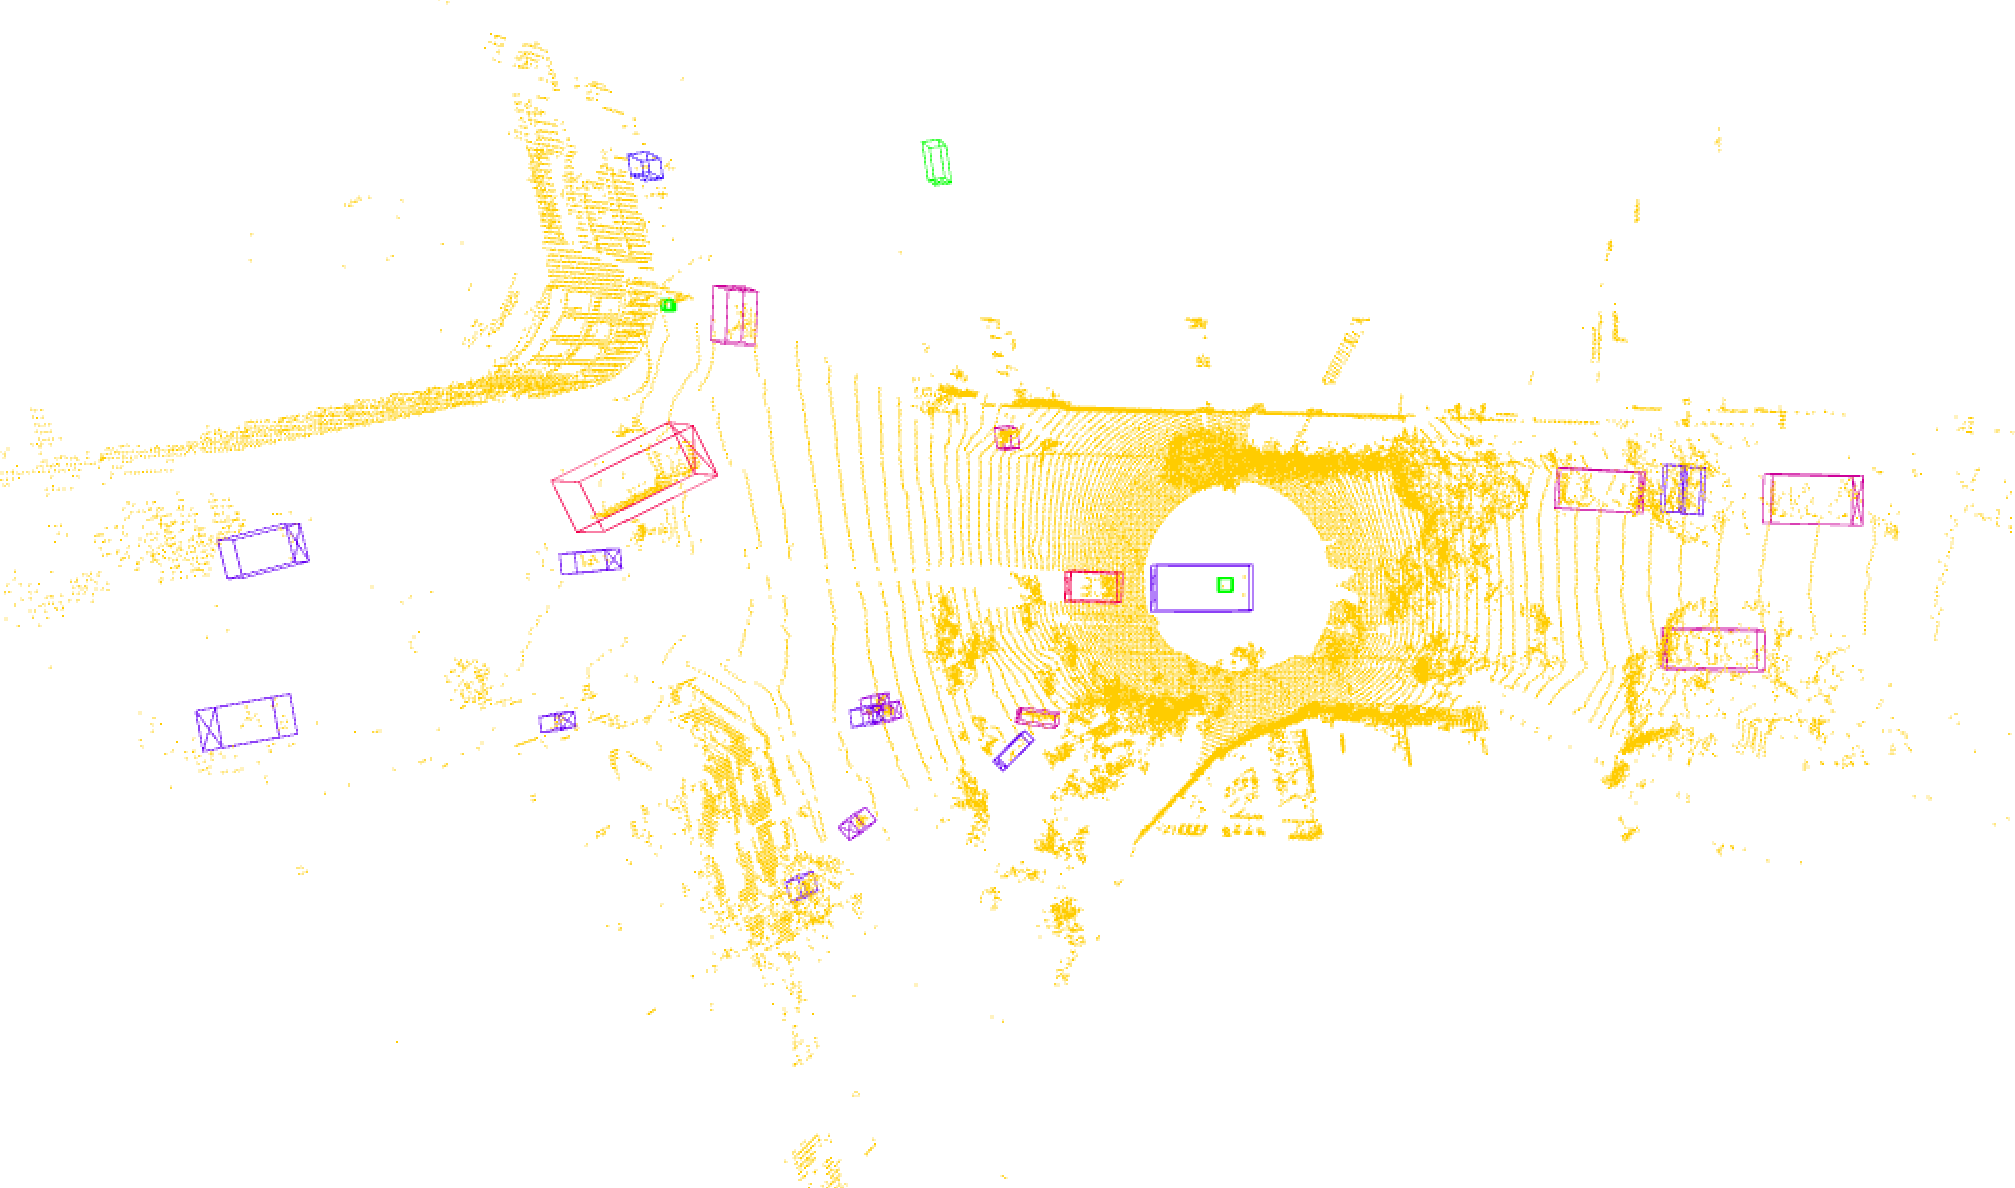
\includegraphics[width=3.70515in,height=2.18429in]{figures/image11.png}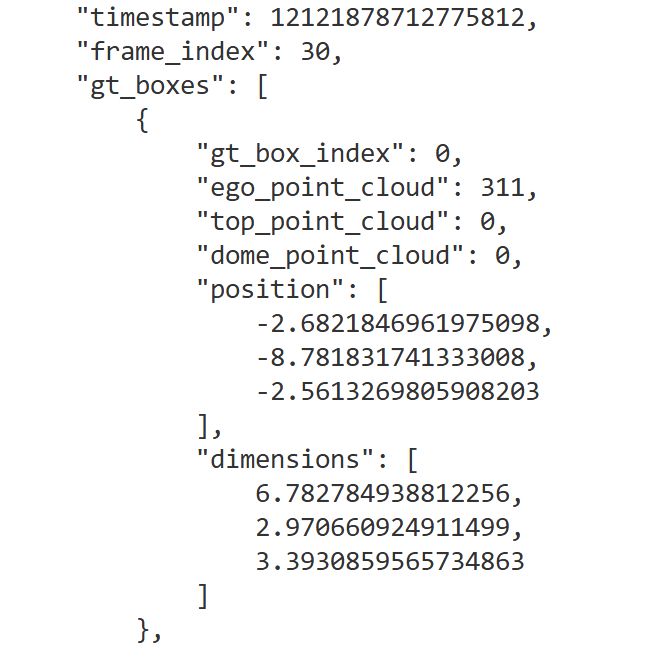
\includegraphics[width=2.25472in,height=2.23063in]{figures/image12.png}

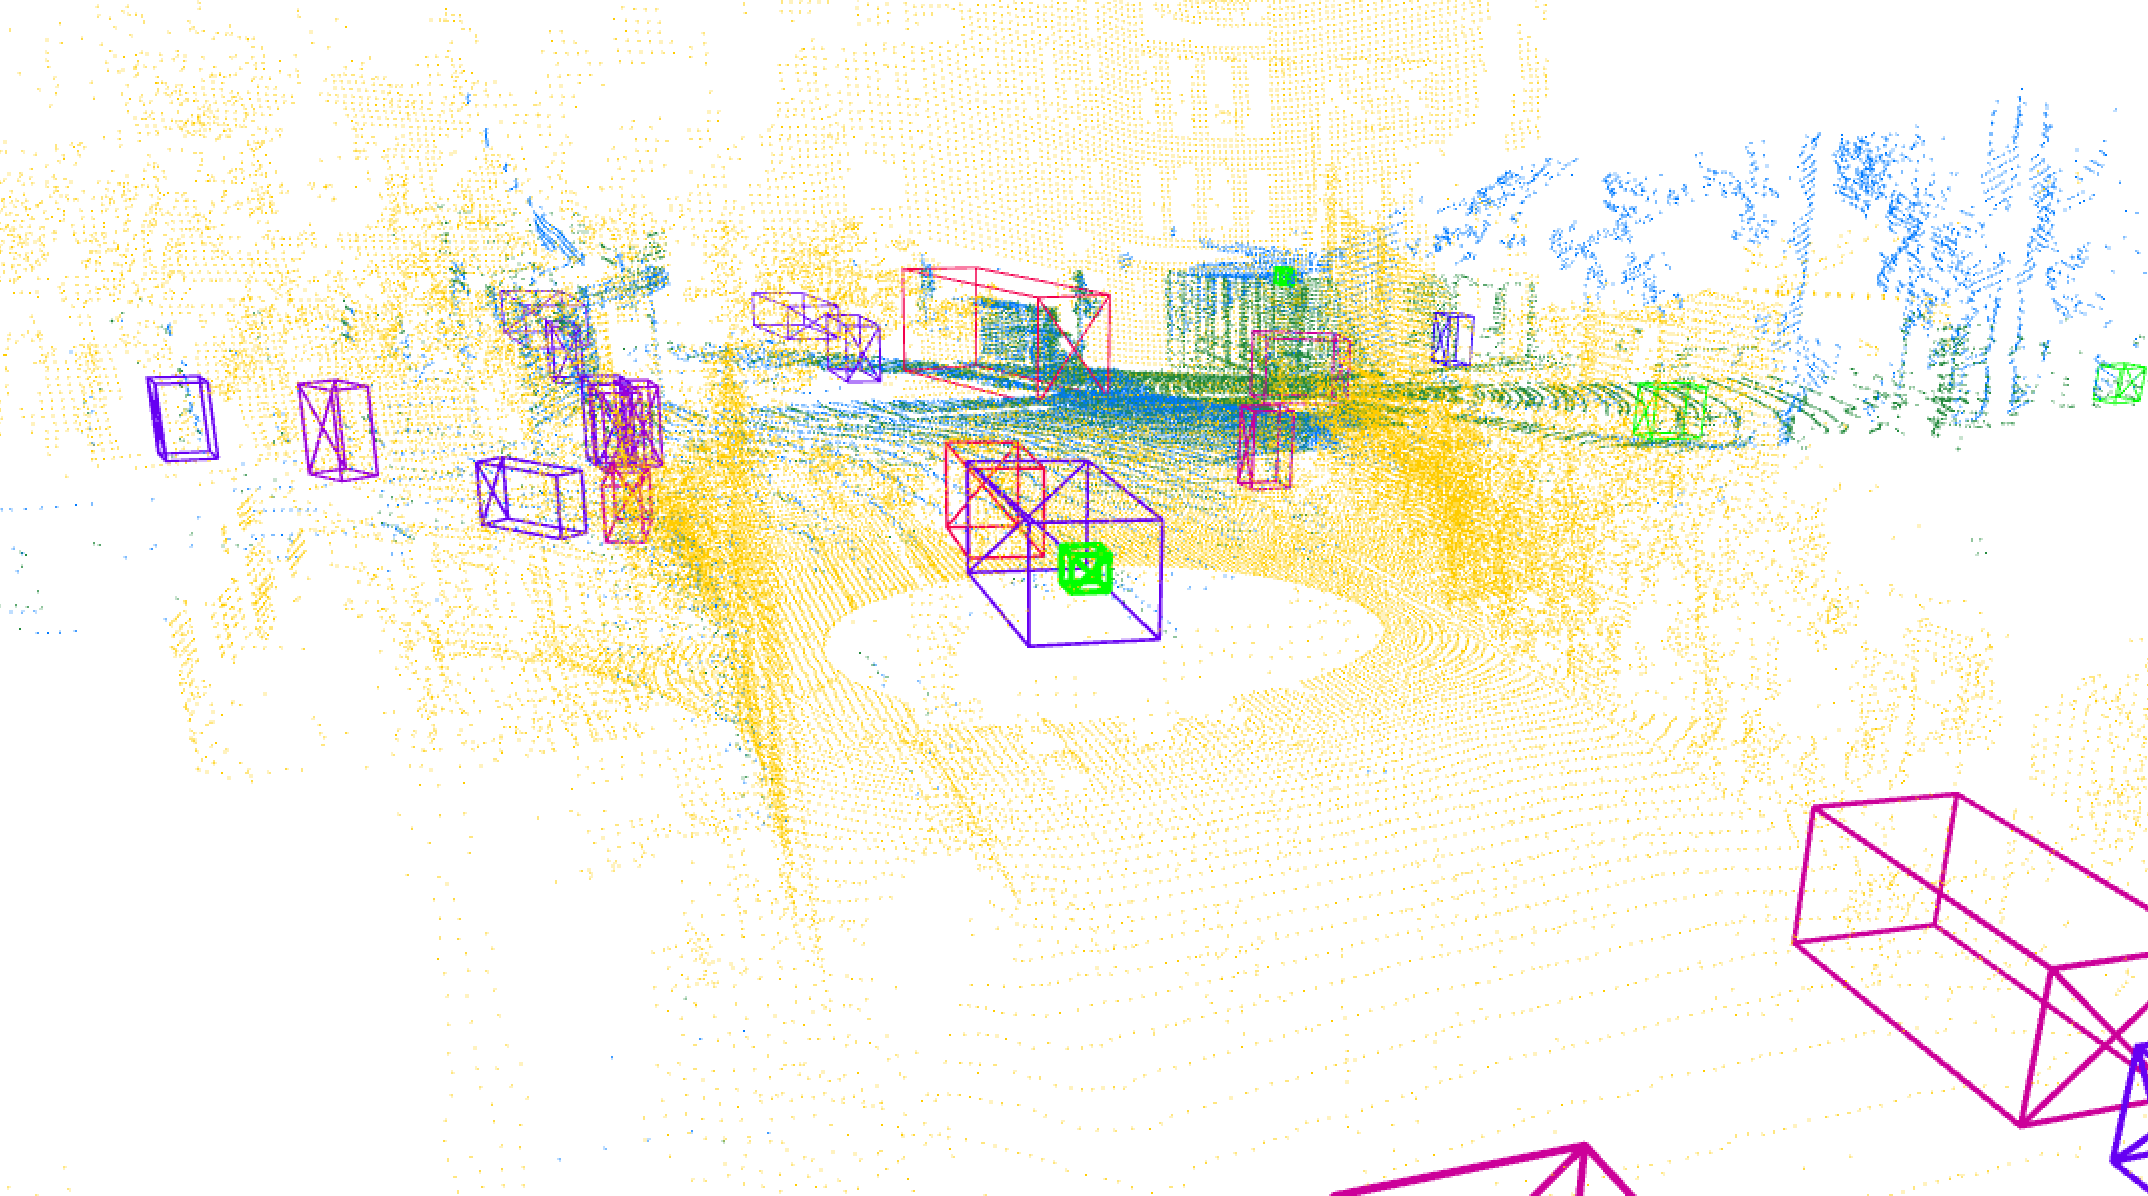
\includegraphics[width=3.32261in,height=1.85015in]{figures/image13.png}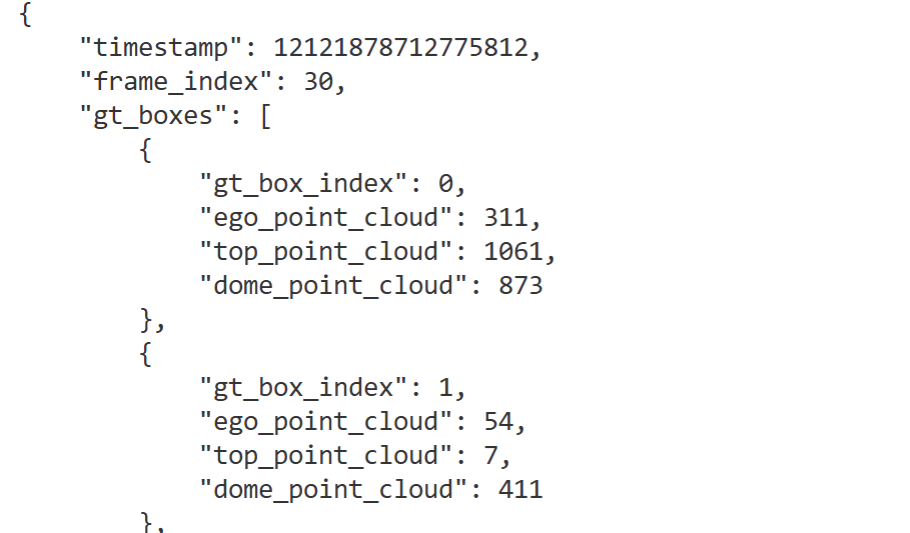
\includegraphics[width=2.22423in,height=1.30293in]{figures/image14.png}

Gathered some basic metrics from the data where I found the number of
intersecting point clouds and ground truth boxes. This gave me some
insights into developing some metrics that I can come up with to
quantify the occlusion.

\begin{enumerate}
\def\labelenumi{\arabic{enumi}.}
\setcounter{enumi}{2}
\item
  \textbf{Data / Results / Plots / Diagrams / Equations}
\end{enumerate}

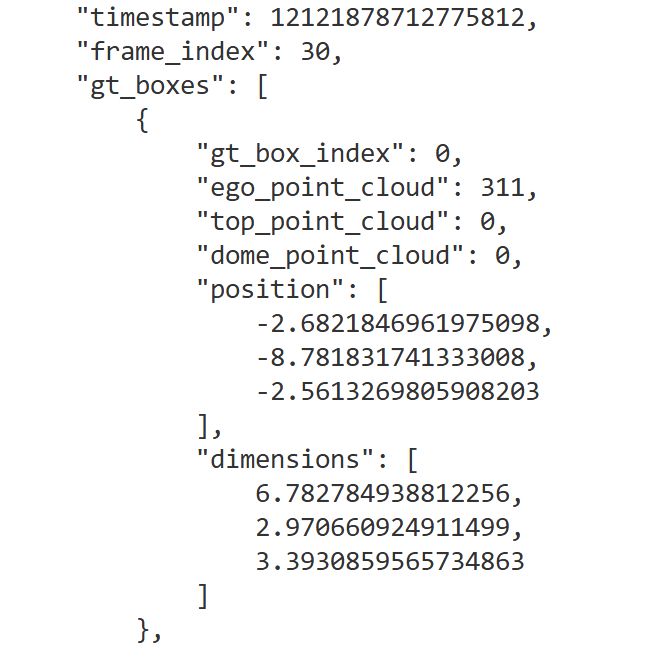
\includegraphics[width=2.25472in,height=2.23063in]{figures/image12.png}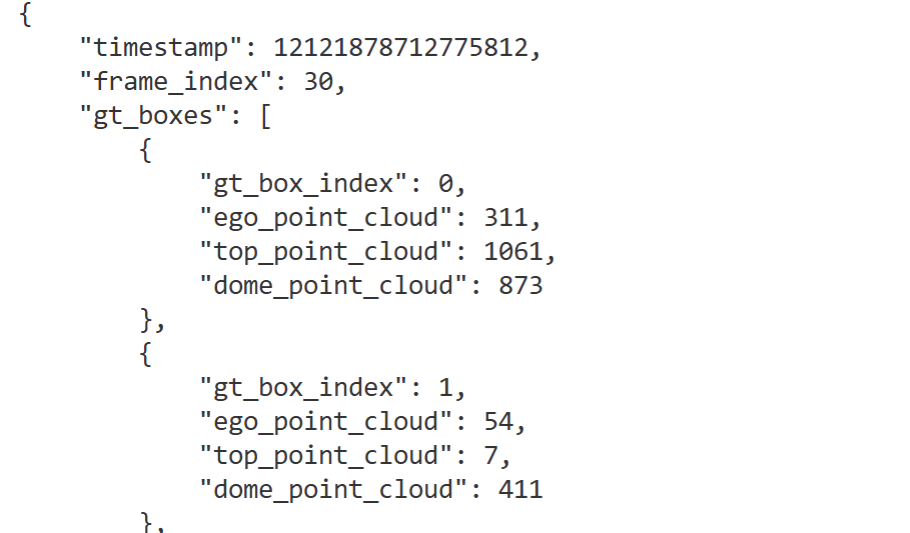
\includegraphics[width=3.37201in,height=1.97529in]{figures/image14.png}

\begin{enumerate}
\def\labelenumi{\arabic{enumi}.}
\setcounter{enumi}{3}
\item
  \textbf{Observations and Reflections}
\end{enumerate}

Some insights that I gained were that it is a good idea to revise the
proposal and come back to it as a reference and change as I go.

\begin{enumerate}
\def\labelenumi{\arabic{enumi}.}
\setcounter{enumi}{4}
\item
  \textbf{Problems Encountered}
\end{enumerate}

n/a

\begin{enumerate}
\def\labelenumi{\arabic{enumi}.}
\setcounter{enumi}{5}
\item
  \textbf{Next Steps / To-Do List (max 50 words)}
\item
\end{enumerate}

Next steps would be to put together a literature review. Also use
endnote to make my source accurate. Use Mendeley.

\begin{enumerate}
\def\labelenumi{\arabic{enumi}.}
\setcounter{enumi}{7}
\item
  \textbf{Appendices / Reference Notes (optional)}
\end{enumerate}

n/a
\end{minipage} \\
\begin{minipage}[t]{\linewidth}\raggedright
\textbf{Weekly/} \textbf{Fortnightly Log Entry}

\textbf{Project Title:} LiDAR Based Occlusion Metric for Autonomous
Vehicles in Urban Environments

\textbf{Supervisor: Mao Shan}

\textbf{Date: 24/04/2026}

\textbf{Meeting Time/s: 10:30-11 AM 24/4/2026}

\textbf{Meeting Minutes:}

\emph{Preliminary Report:}

Ordering: lidar, datasets, 3d object detection, detection metrics,
occlusion, occlusion metrics,

\begin{itemize}
\item
  Have a look into categories of detectors, ie voxel based or point
  based
\item
  Include labelling criterias for datasets
\item
  Aim to design for performance differences;
\end{itemize}

Deliverables / Scope:

\begin{itemize}
\item
  1. Occlusion Metrics
\item
  2. Experiment design: 1 dataset , 1 method / approach
\end{itemize}

Position of metrics:

\begin{itemize}
\item
  1. Supplement accurate labelling
\item
  2. Optimisation of LiDAR deployment
\item
  3. Improve the 3D detection benchmarking
\end{itemize}

V2X -- methods for novelty

\begin{itemize}
\item
  Not communication based but perhaps fusion
\end{itemize}

\begin{enumerate}
\def\labelenumi{\arabic{enumi}.}
\setcounter{enumi}{7}
\item
  \textbf{Objectives}
\end{enumerate}

n/a

\begin{itemize}
\item
  Discussed Mixed Signals and Possible paths to go down with Mixed
  Signals
\item
  Cooperative Perception, Predictive Perception,
\end{itemize}

\begin{enumerate}
\def\labelenumi{\arabic{enumi}.}
\setcounter{enumi}{8}
\item
  \textbf{Activities Performed}
\end{enumerate}

Handed in the first draft of the Prelim report/ literature review

\begin{enumerate}
\def\labelenumi{\arabic{enumi}.}
\setcounter{enumi}{9}
\item
  \textbf{Data / Results / Plots / Diagrams / Equations}
\end{enumerate}

n/a

\begin{enumerate}
\def\labelenumi{\arabic{enumi}.}
\setcounter{enumi}{10}
\item
  \textbf{Observations and Reflections}
\end{enumerate}

n/a

\begin{enumerate}
\def\labelenumi{\arabic{enumi}.}
\setcounter{enumi}{11}
\item
  \textbf{Problems Encountered}
\end{enumerate}

\begin{itemize}
\item
  Focus on the scope of the study
\item
  Problem for the metric? Is it for lidar optimization, sensor
  deployment or dataset benchtesting
\end{itemize}

Focus on what is assumed in the study as well

\begin{enumerate}
\def\labelenumi{\arabic{enumi}.}
\setcounter{enumi}{12}
\item
  \textbf{Next Steps / To-Do List (max 50 words)}
\end{enumerate}

n/a

\begin{enumerate}
\def\labelenumi{\arabic{enumi}.}
\setcounter{enumi}{13}
\item
  \textbf{Appendices / Reference Notes (optional)}
\end{enumerate}

n/a
\end{minipage} \\
\begin{minipage}[t]{\linewidth}\raggedright
\textbf{Weekly/} \textbf{Fortnightly Log Entry}

\textbf{Project Title: Machine Learning Models using the Mixed Signals
Dataset}

\textbf{Supervisor: Mao Shan}

\textbf{Meeting Time: Week 10 5\textsuperscript{th} May 10:30 AM,}

\begin{enumerate}
\def\labelenumi{\arabic{enumi}.}
\item
  \textbf{Objectives}
\end{enumerate}

n/a

Overseas Meeting Discussed the next couple of meetings, what to be
expected from a seminar and prelim report.

\begin{enumerate}
\def\labelenumi{\arabic{enumi}.}
\setcounter{enumi}{1}
\item
  \textbf{Activities Performed}
\end{enumerate}

n/a

\begin{enumerate}
\def\labelenumi{\arabic{enumi}.}
\setcounter{enumi}{2}
\item
  \textbf{Data / Results / Plots / Diagrams / Equations}
\end{enumerate}

n/a

\begin{enumerate}
\def\labelenumi{\arabic{enumi}.}
\setcounter{enumi}{3}
\item
  \textbf{Observations and Reflections}
\end{enumerate}

n/a

\begin{enumerate}
\def\labelenumi{\arabic{enumi}.}
\setcounter{enumi}{4}
\item
  \textbf{Problems Encountered}
\end{enumerate}

Any bugs, hardware issues, theoretical blocks, etc. (max 50 words)

\begin{enumerate}
\def\labelenumi{\arabic{enumi}.}
\setcounter{enumi}{5}
\item
  \textbf{Next Steps / To-Do List (max 50 words)}
\end{enumerate}

n/a

\begin{enumerate}
\def\labelenumi{\arabic{enumi}.}
\setcounter{enumi}{6}
\item
  \textbf{Appendices / Reference Notes (optional)}
\end{enumerate}

n/a
\end{minipage} \\
\begin{minipage}[t]{\linewidth}\raggedright
\textbf{Weekly/} \textbf{Fortnightly Log Entry}

\textbf{Project Title:} LiDAR Based Occlusion Metric for 3D Object
Perception in Urban Environments

\textbf{Supervisor: Mao Shan}

\textbf{Meeting Time: Week 11 Meeting 15\textsuperscript{th} May Friday,
Week 12 Meeting 22\textsuperscript{nd} May}

\begin{enumerate}
\def\labelenumi{\arabic{enumi}.}
\item
  \textbf{Objectives}
\end{enumerate}

n/a

Review of the Slides, make the topic more general less focused on
camera-bias.

Keep working on Preliminary Report

\begin{enumerate}
\def\labelenumi{\arabic{enumi}.}
\setcounter{enumi}{1}
\item
  \textbf{Activities Performed}
\end{enumerate}

Change of the title. Develop methodologies and some baseline metrics
that can be used.

\begin{enumerate}
\def\labelenumi{\arabic{enumi}.}
\setcounter{enumi}{2}
\item
  \textbf{Data / Results / Plots / Diagrams / Equations}
\end{enumerate}

n/a

\begin{enumerate}
\def\labelenumi{\arabic{enumi}.}
\setcounter{enumi}{3}
\item
  \textbf{Observations and Reflections}
\end{enumerate}

n/a

\begin{enumerate}
\def\labelenumi{\arabic{enumi}.}
\setcounter{enumi}{4}
\item
  \textbf{Problems Encountered}
\end{enumerate}

n/a

\begin{enumerate}
\def\labelenumi{\arabic{enumi}.}
\setcounter{enumi}{5}
\item
  \textbf{Next Steps / To-Do List (max 50 words)}
\end{enumerate}

n/a

\begin{enumerate}
\def\labelenumi{\arabic{enumi}.}
\setcounter{enumi}{6}
\item
  \textbf{Appendices / Reference Notes (optional)}
\end{enumerate}

n/a
\end{minipage} \\
\end{longtable}

\end{document}
